\documentclass[UFT8]{ctexart}%\setcounter{page}{1}
\setCJKmainfont[BoldFont=STHeiti,ItalicFont=STKaiti]{STSong}%\fangsong \songti  \heiti \kaishu \wuhao \small \large \LARGE
\usepackage{graphicx} % 导入插图功能
\usepackage{float}
\usepackage{threeparttable}
\usepackage{caption}
\usepackage{subfigure}
\usepackage{amsmath}
\usepackage{diagbox} % \diagbox[斜线方形]{分区1内容}{分区2内容}{分区3内容}...
\usepackage{ulem}
\usepackage{ctex}
\usepackage{booktabs}% \toprule \midrule \bottomrule
\usepackage{multirow}% \multicolumn{}{}{}
\usepackage{ulem}%\xout 斜删除线 \sout 删除线 \uline下划线 \uuline 双下划线 \uwave 波浪线 
 \usepackage{geometry} \geometry{a4paper}
\usepackage{graphicx}

\newcommand\mydot[1]{\scalebox{#1}{.}}
%\renewcommand\cftdot{\mydot{0.8}} % change the size of dots
%\renewcommand\cftdotsep{3} % change the space between dots


\usepackage{pdfpages}%\includepdf[pages=-]{插入的文件.pdf} 
%\usepackage[final]{pdfpages} %\includepdf{figure.pdf} 

\usepackage{color}
\def\red{\textcolor{red}}
\def\blue{\textcolor{blue}}
\definecolor{green}{RGB}{0,153,51}
\def\green{\textcolor{green}}

\def\bi{\begin{itemize}}
\def\ei{\end{itemize}}
\def\be{ \begin{enumerate}}
\def\ee{ \end{enumerate}}

\usepackage{hyperref}% \url \href
\hypersetup{
    colorlinks=true,
    linkcolor=blue,
    filecolor=blue,
    urlcolor=blue,
    pdftitle={Overleaf Example},
%    pdfpagemode=FullScreen,
    }
\urlstyle{same}
\def\link{\hyperlink}
\def\target{\hypertarget}


%\headsep 0.5 true cm \topmargin 0pt \oddsidemargin 0pt
%\evensidemargin -10pt \textheight 297mm \textwidth 210mm

\begin{document}
%\pagestyle{empty}%全部页码为空
\thispagestyle{empty} %该页页码为空
\vspace*{3cm}
\begin{center}
{{\LARGE\heiti 2023年湘潭市建元中学报名材料}\\[0.6cm]
{\normalsize 唐洁}\\[0.1cm]
{\small(广西师范大学数学与统计学院, 广西桂林, 541004)}}
\end{center}

\clearpage%新的一页
%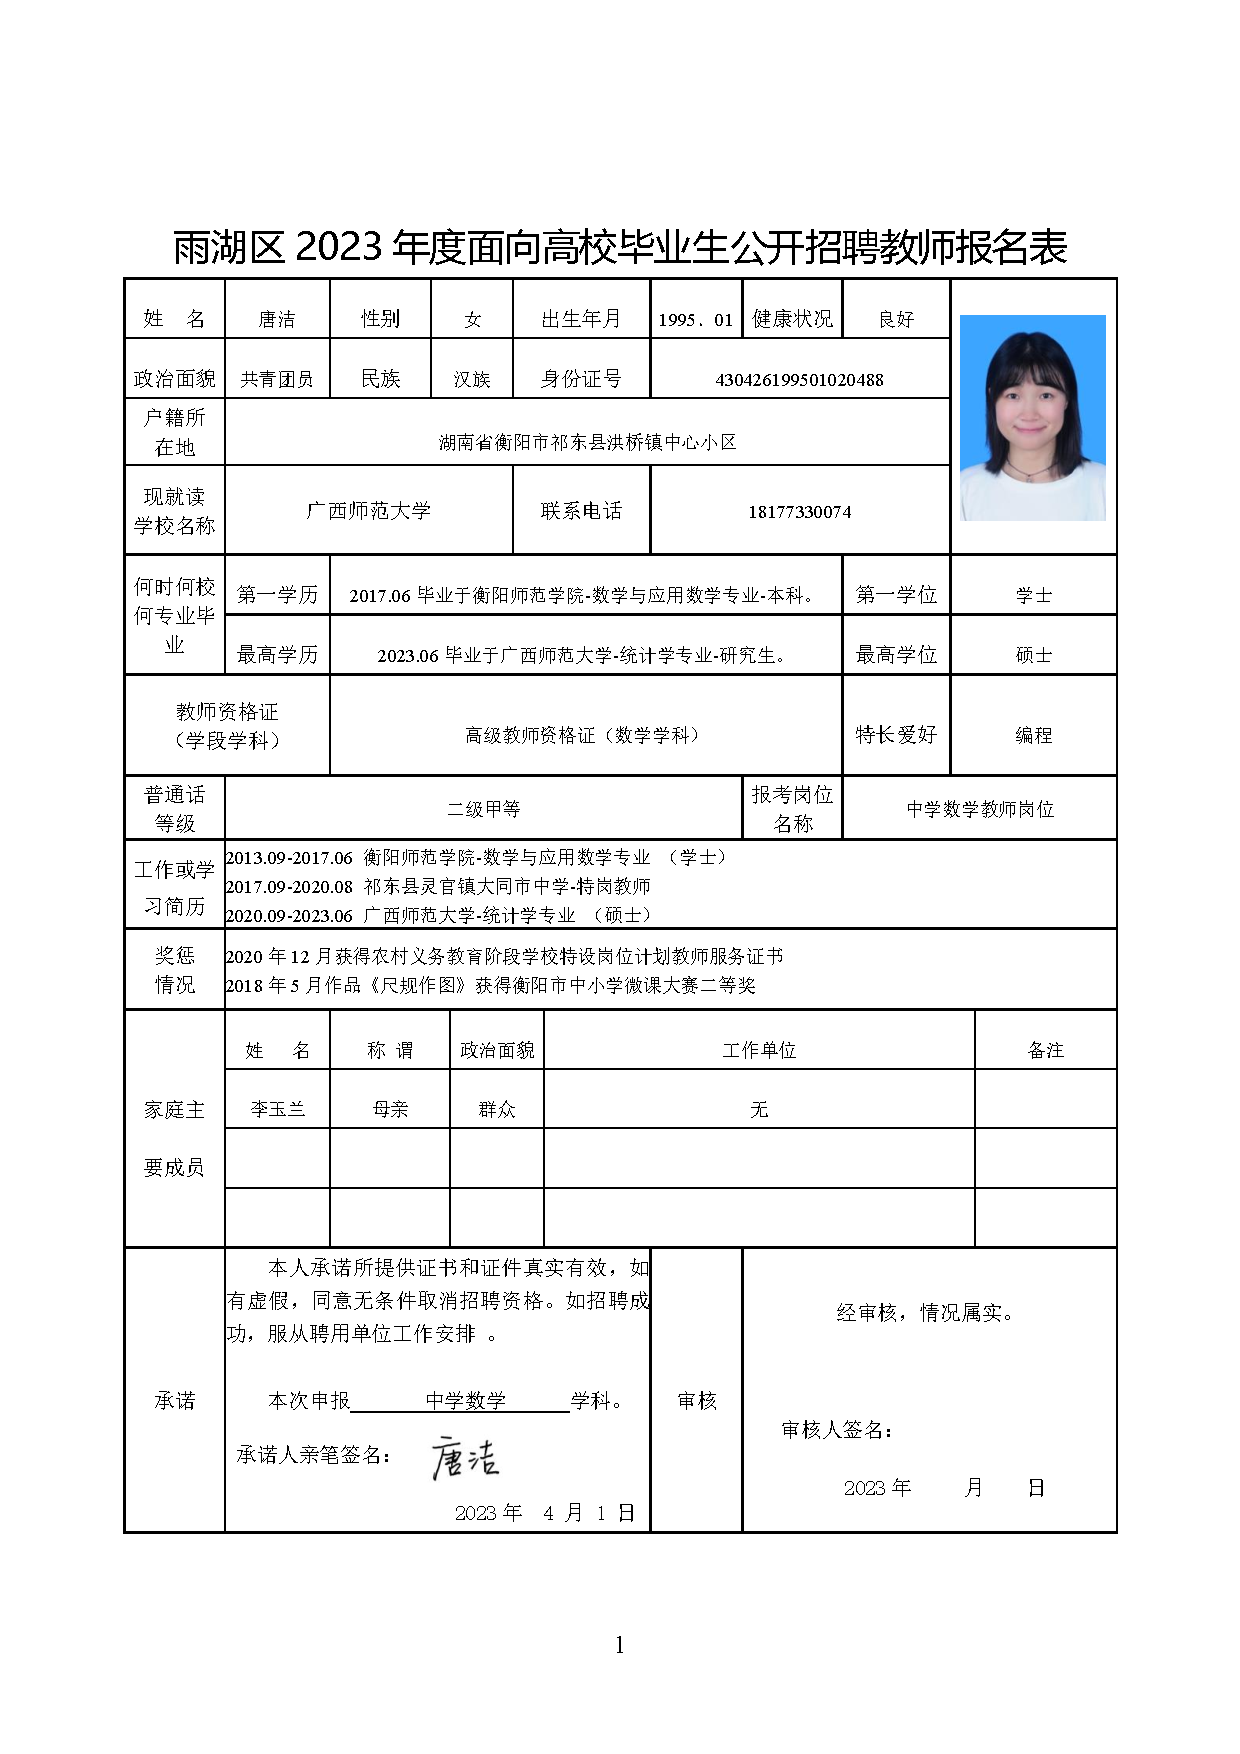
\includepdf[pages=1]{pdfs/湘潭建元中学报名表.pdf}

\tableofcontents%输出目录
\thispagestyle{empty} % 当前页不显示页码

\clearpage%新的一页
\setcounter{page}{1}%设置首页

%
\includepdf[pages=1-3]{唐洁简历.pdf}

\section{身份证}
\begin{center}
  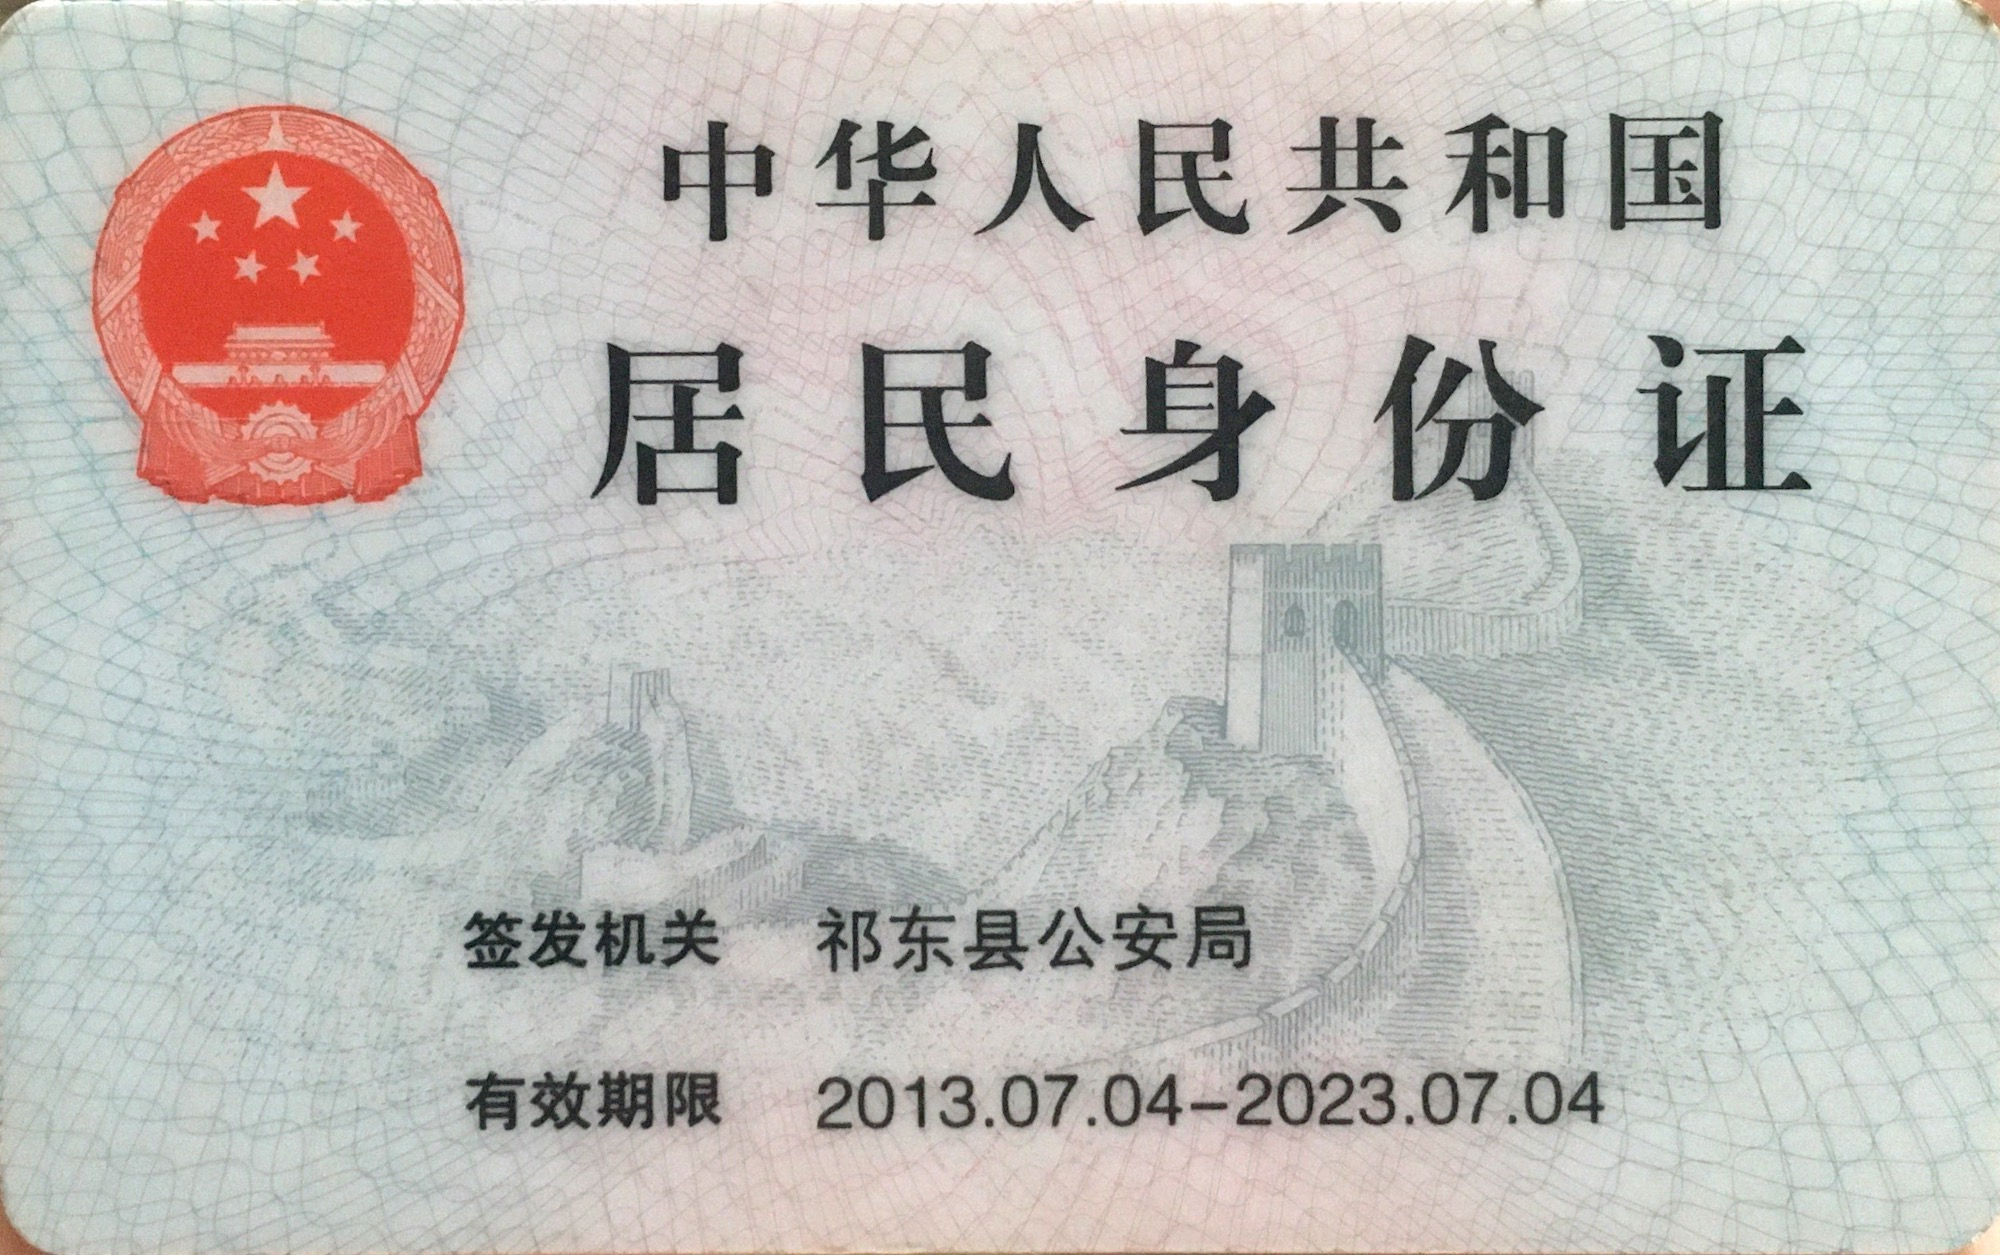
\includegraphics[scale=0.1]{figs/身份证1.JPG }
  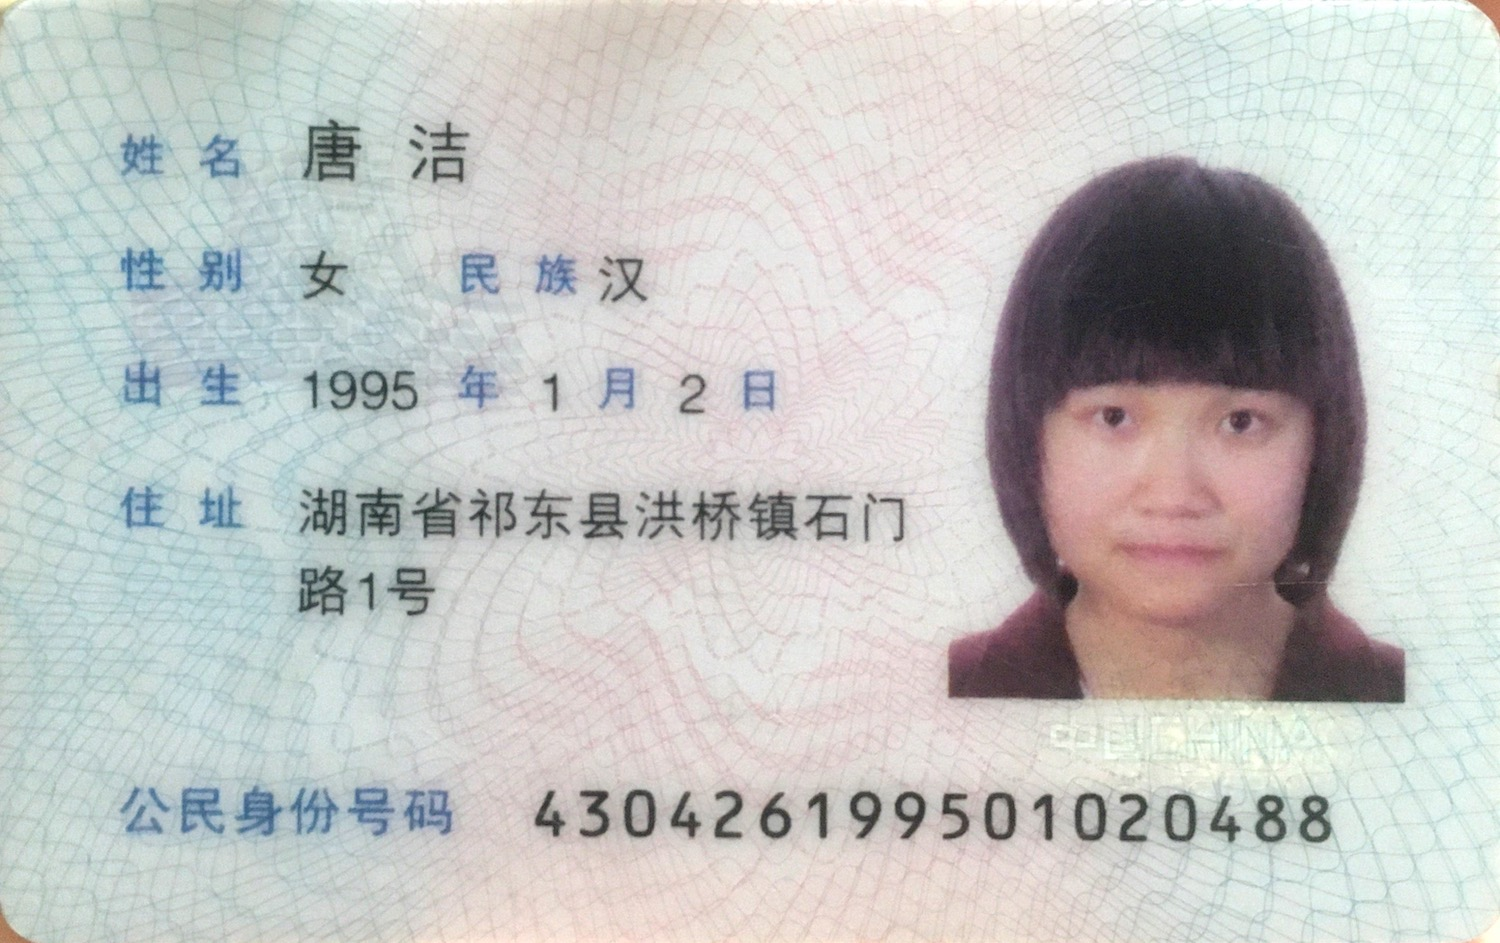
\includegraphics[scale=0.1]{figs/身份证2.JPG }
\end{center}

\section{学生证}
\begin{center}
  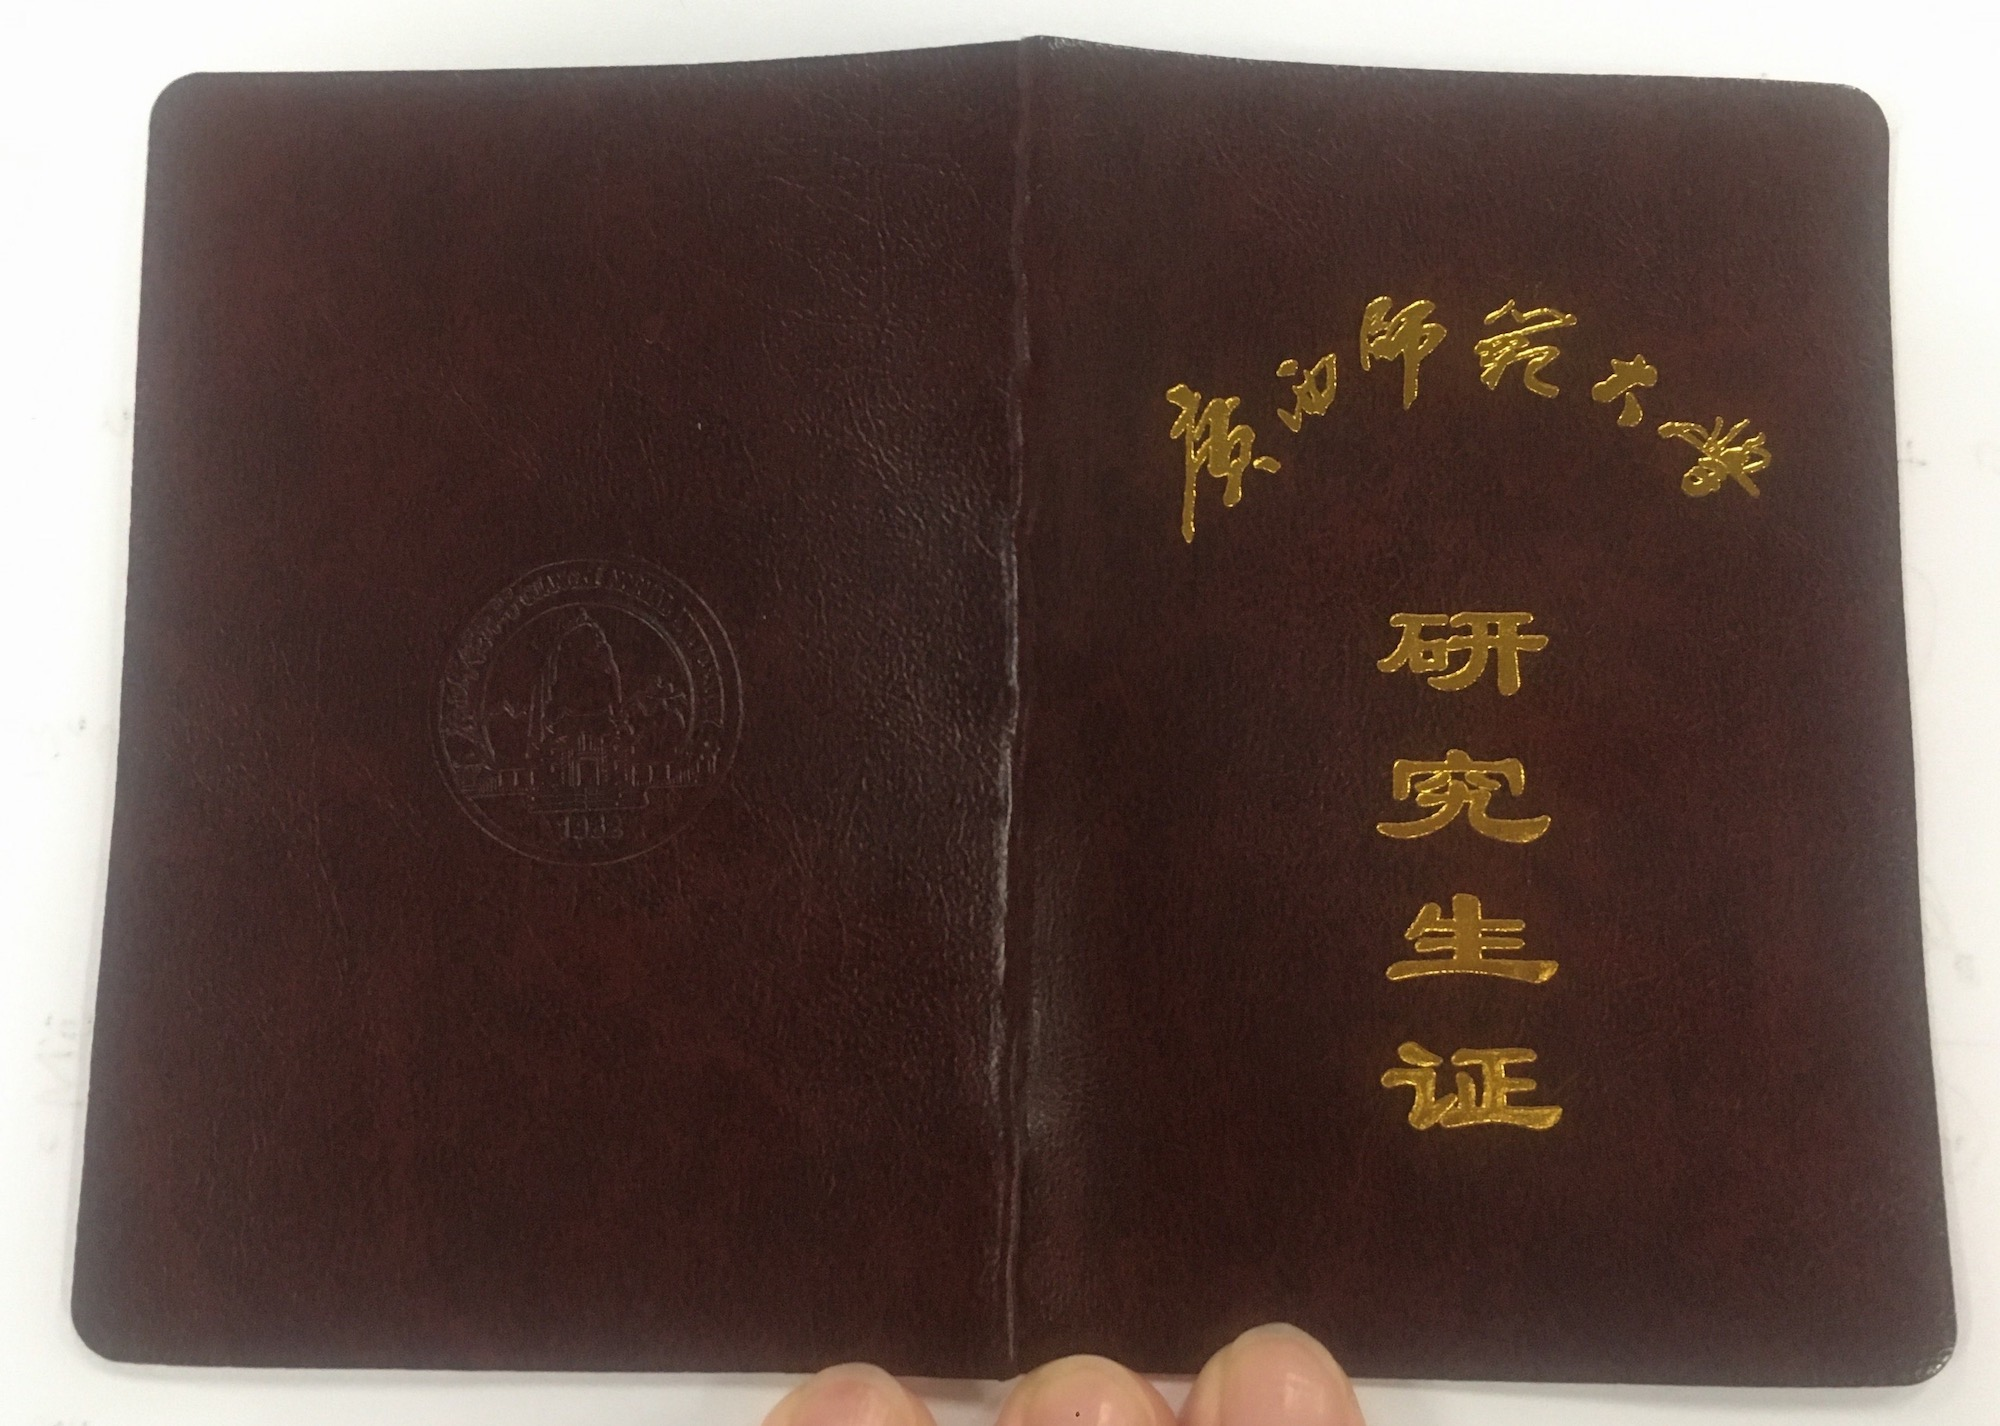
\includegraphics[scale=0.1]{figs/学生证1.JPG }
  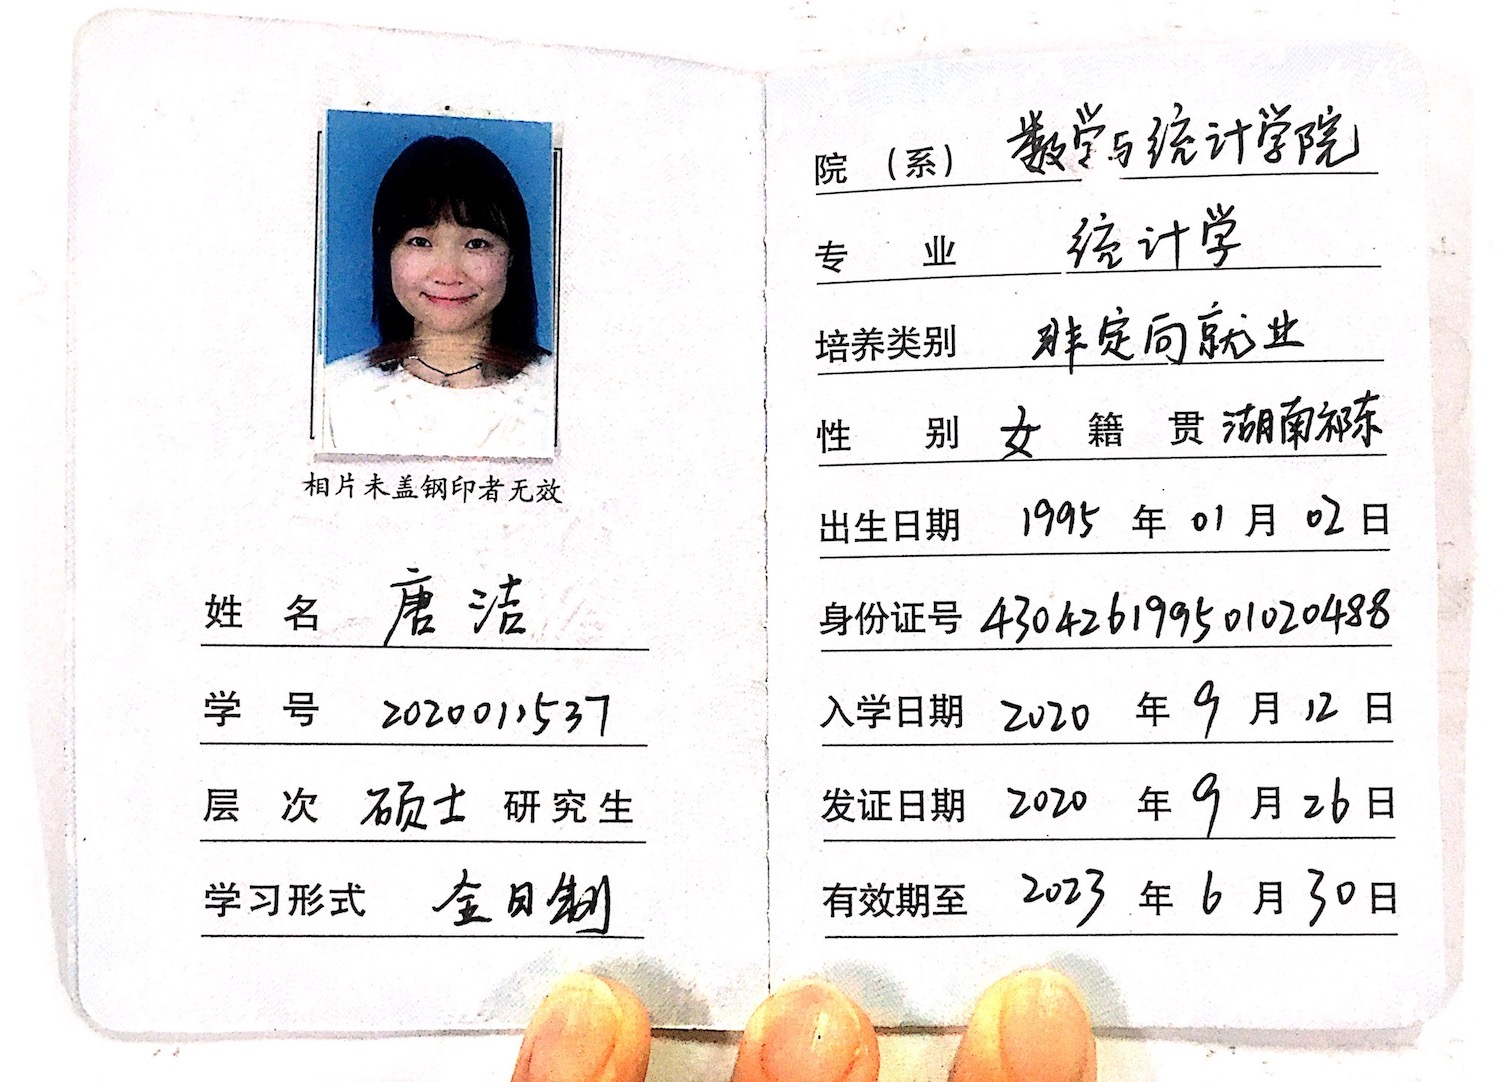
\includegraphics[scale=0.1]{figs/学生证2.JPG }
  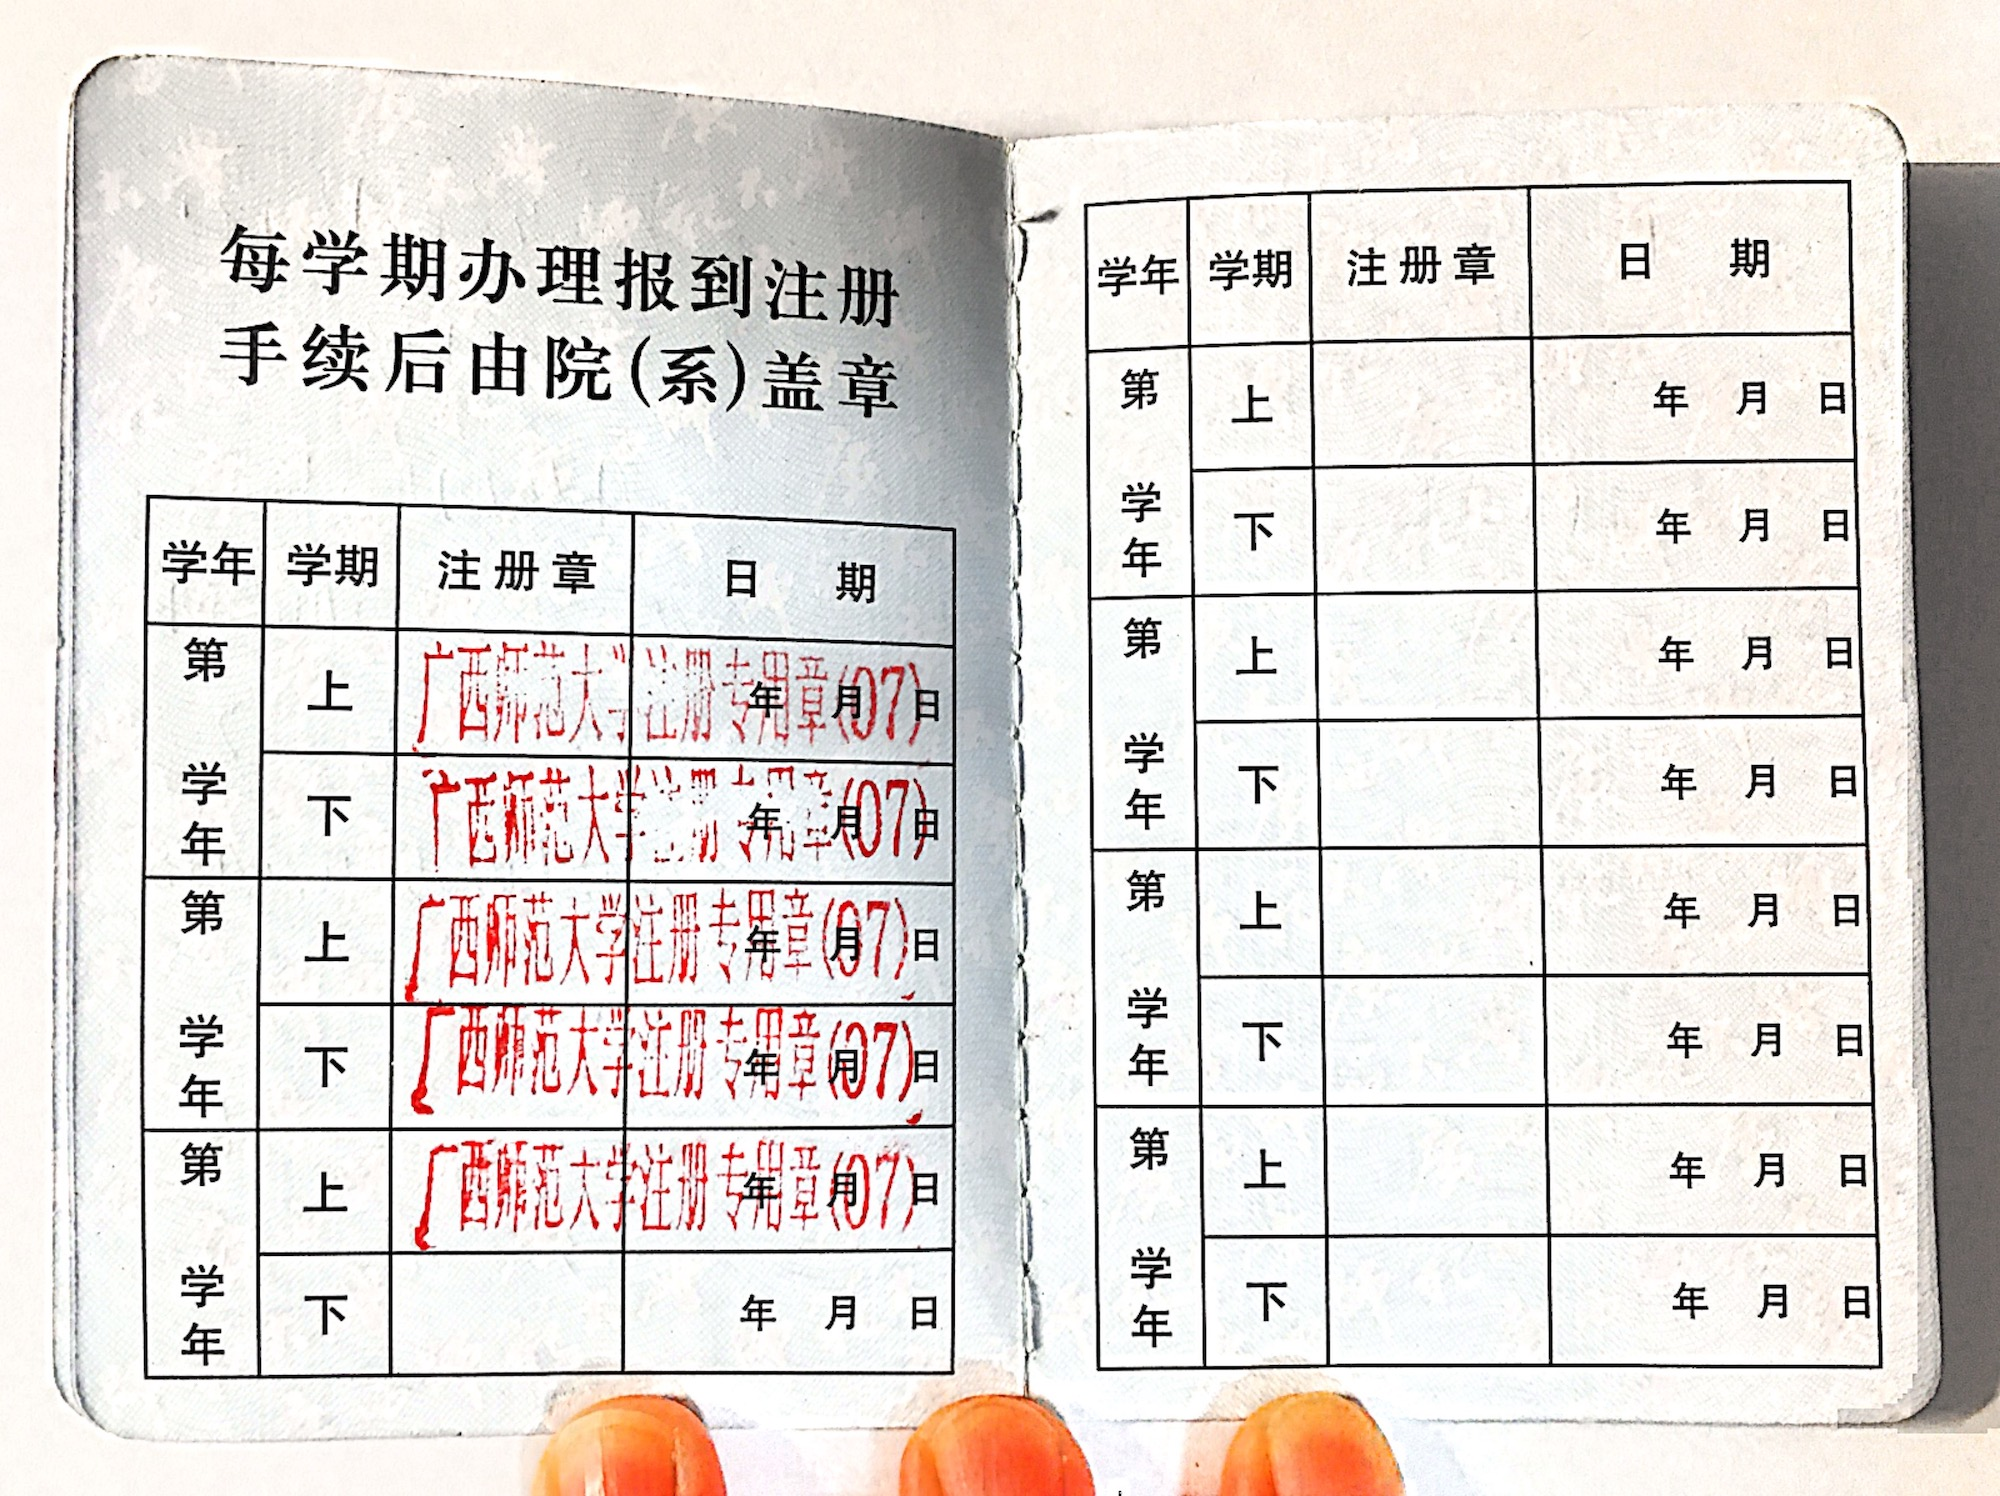
\includegraphics[scale=0.1]{figs/学生证3.JPG }
\end{center}

\section{学历证明}
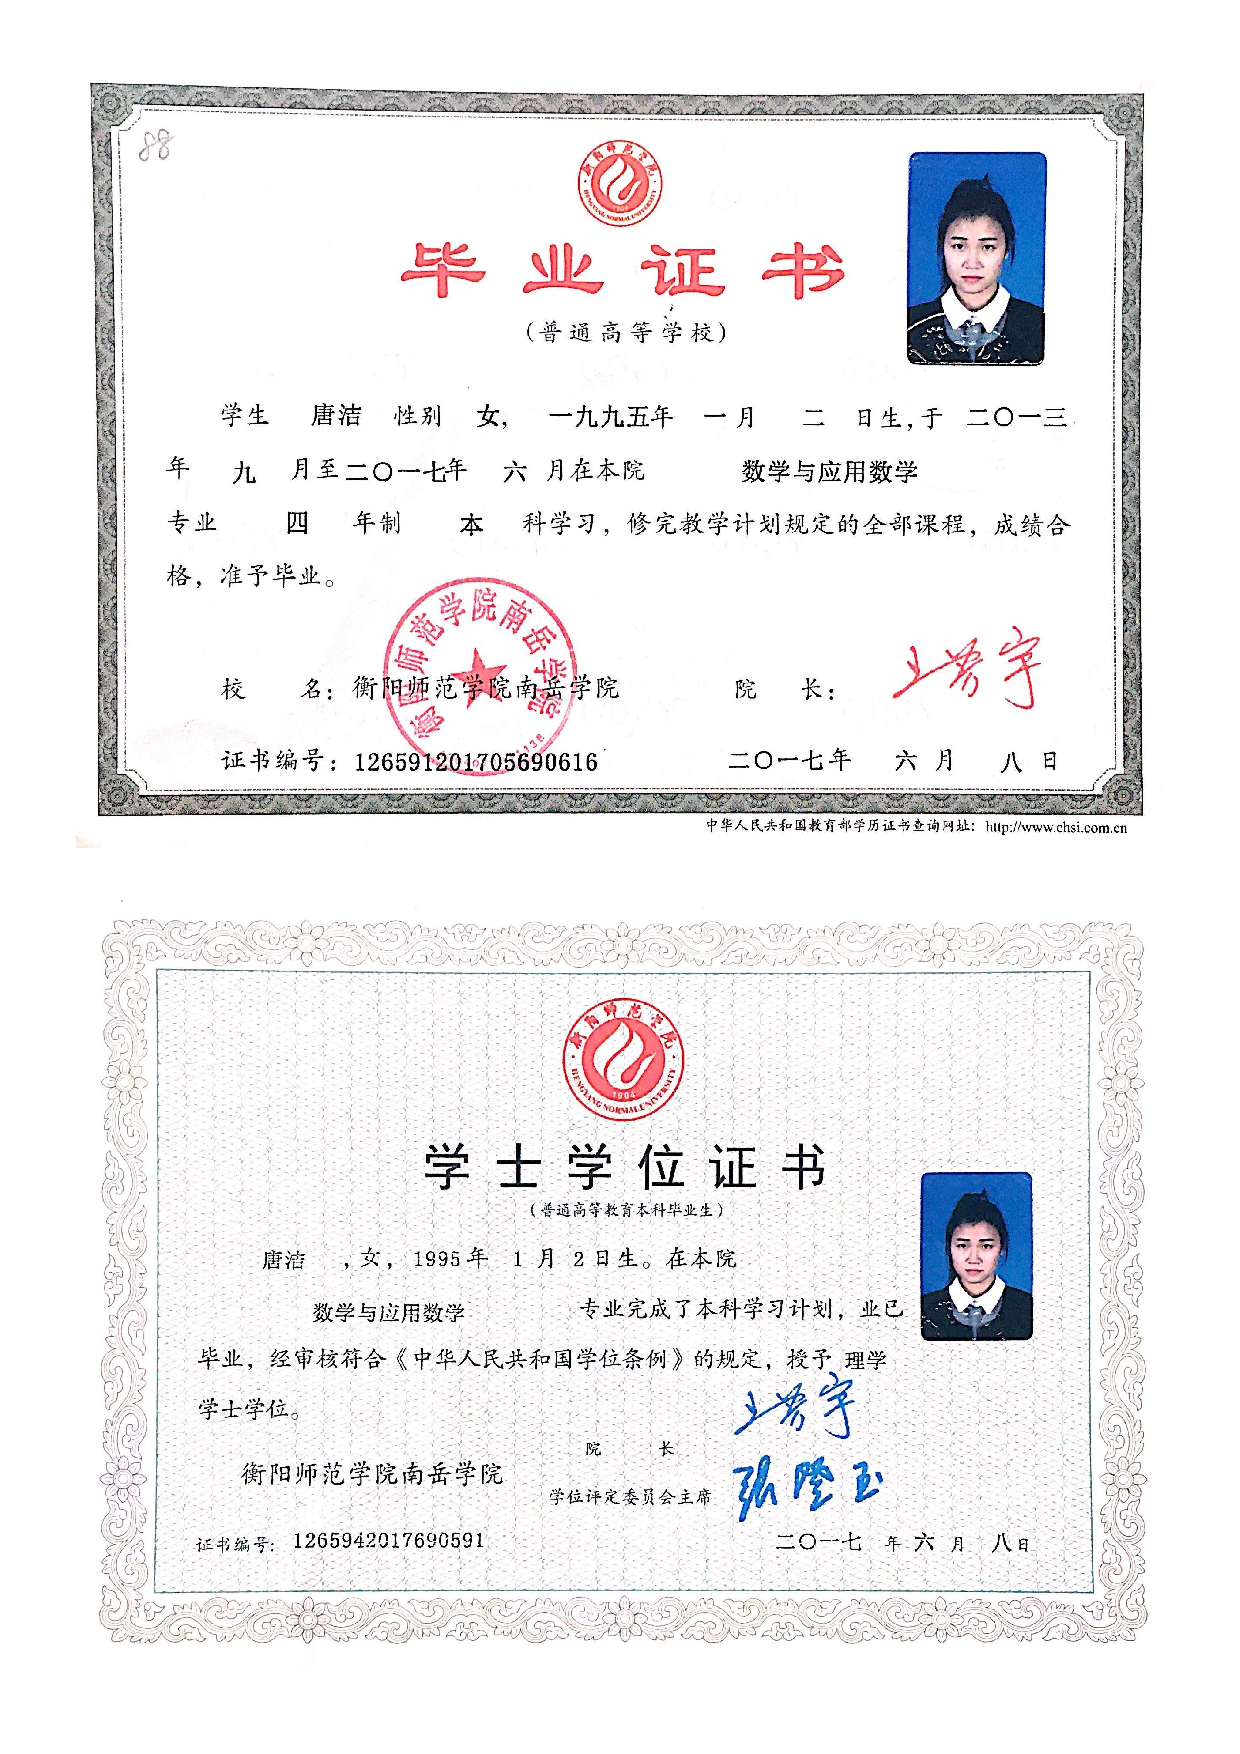
\includepdf[pages=1]{pdfs/本科毕业证与学位证.pdf}
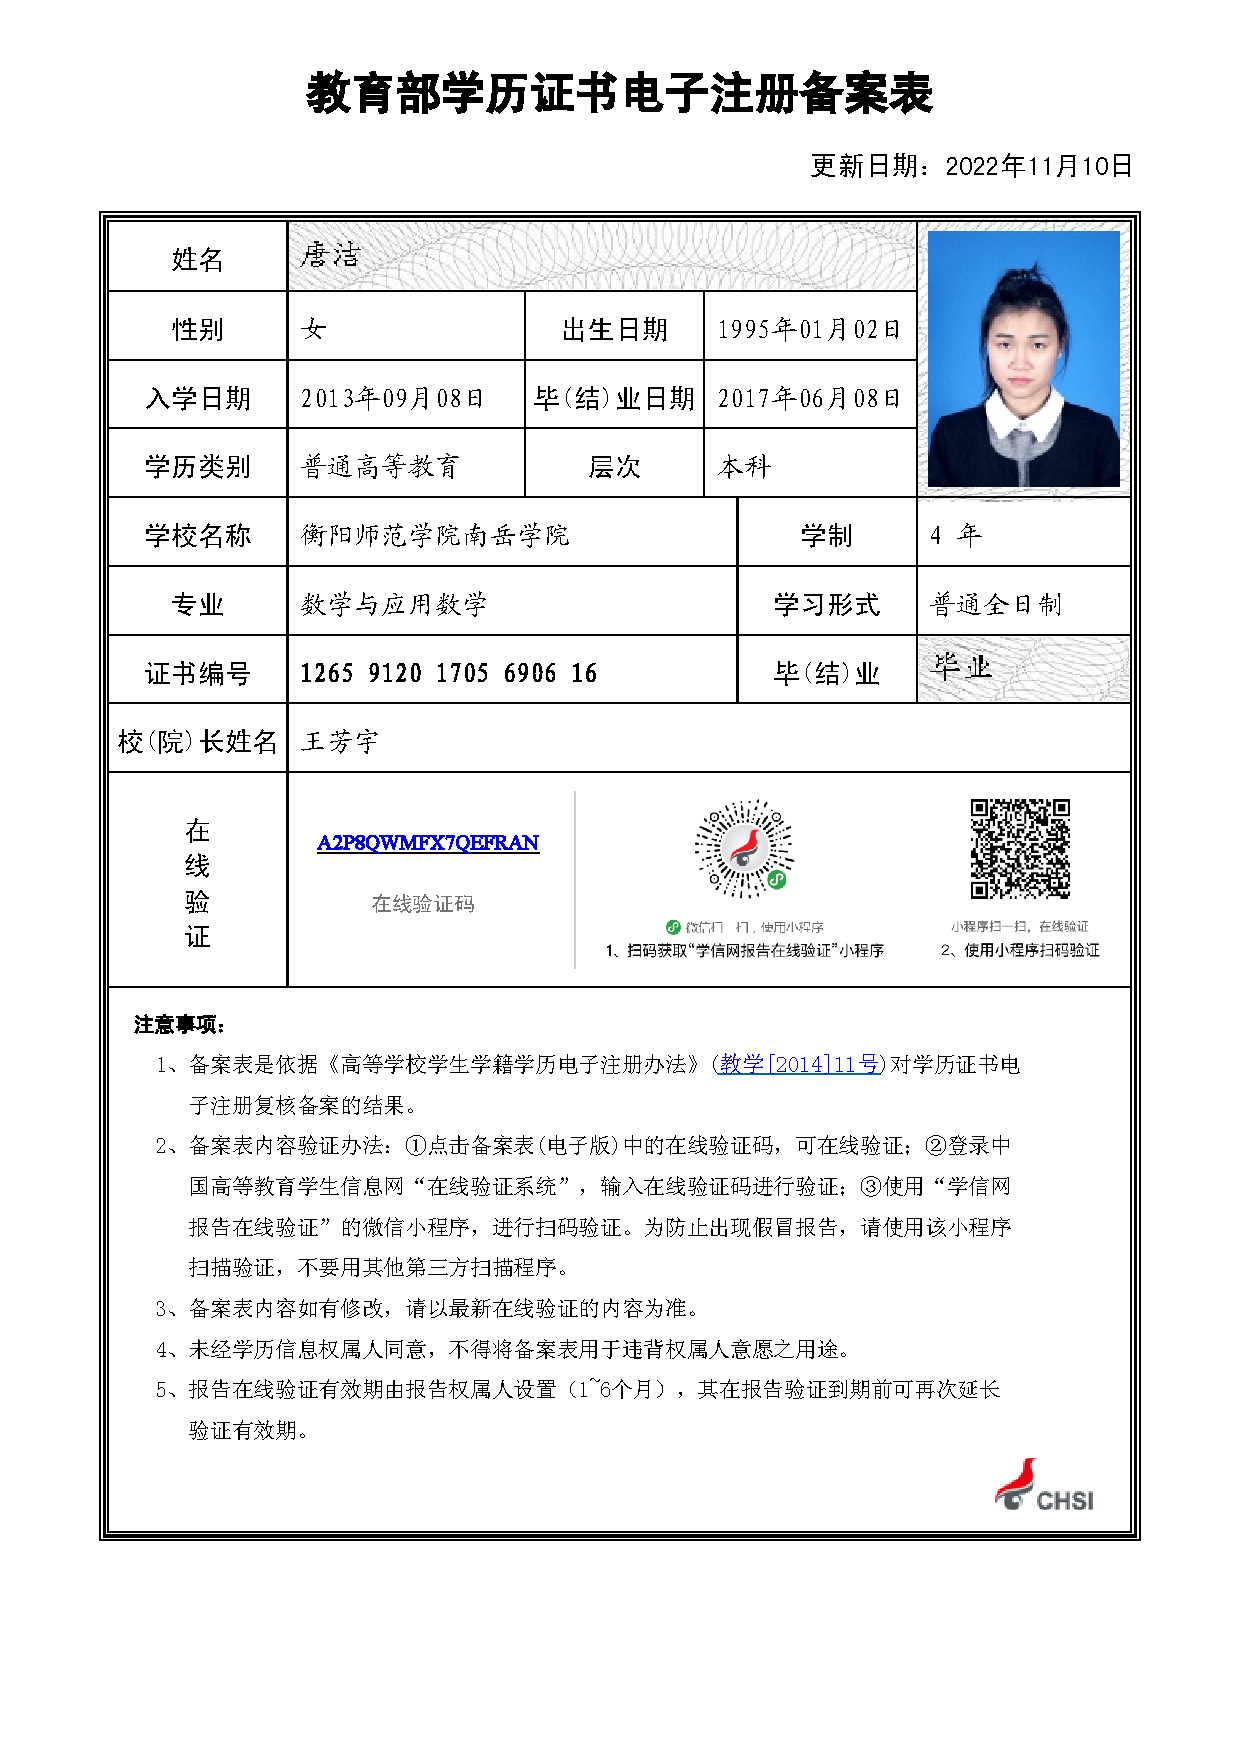
\includepdf[pages=1]{pdfs/教育部学历证书电子注册备案表.pdf}
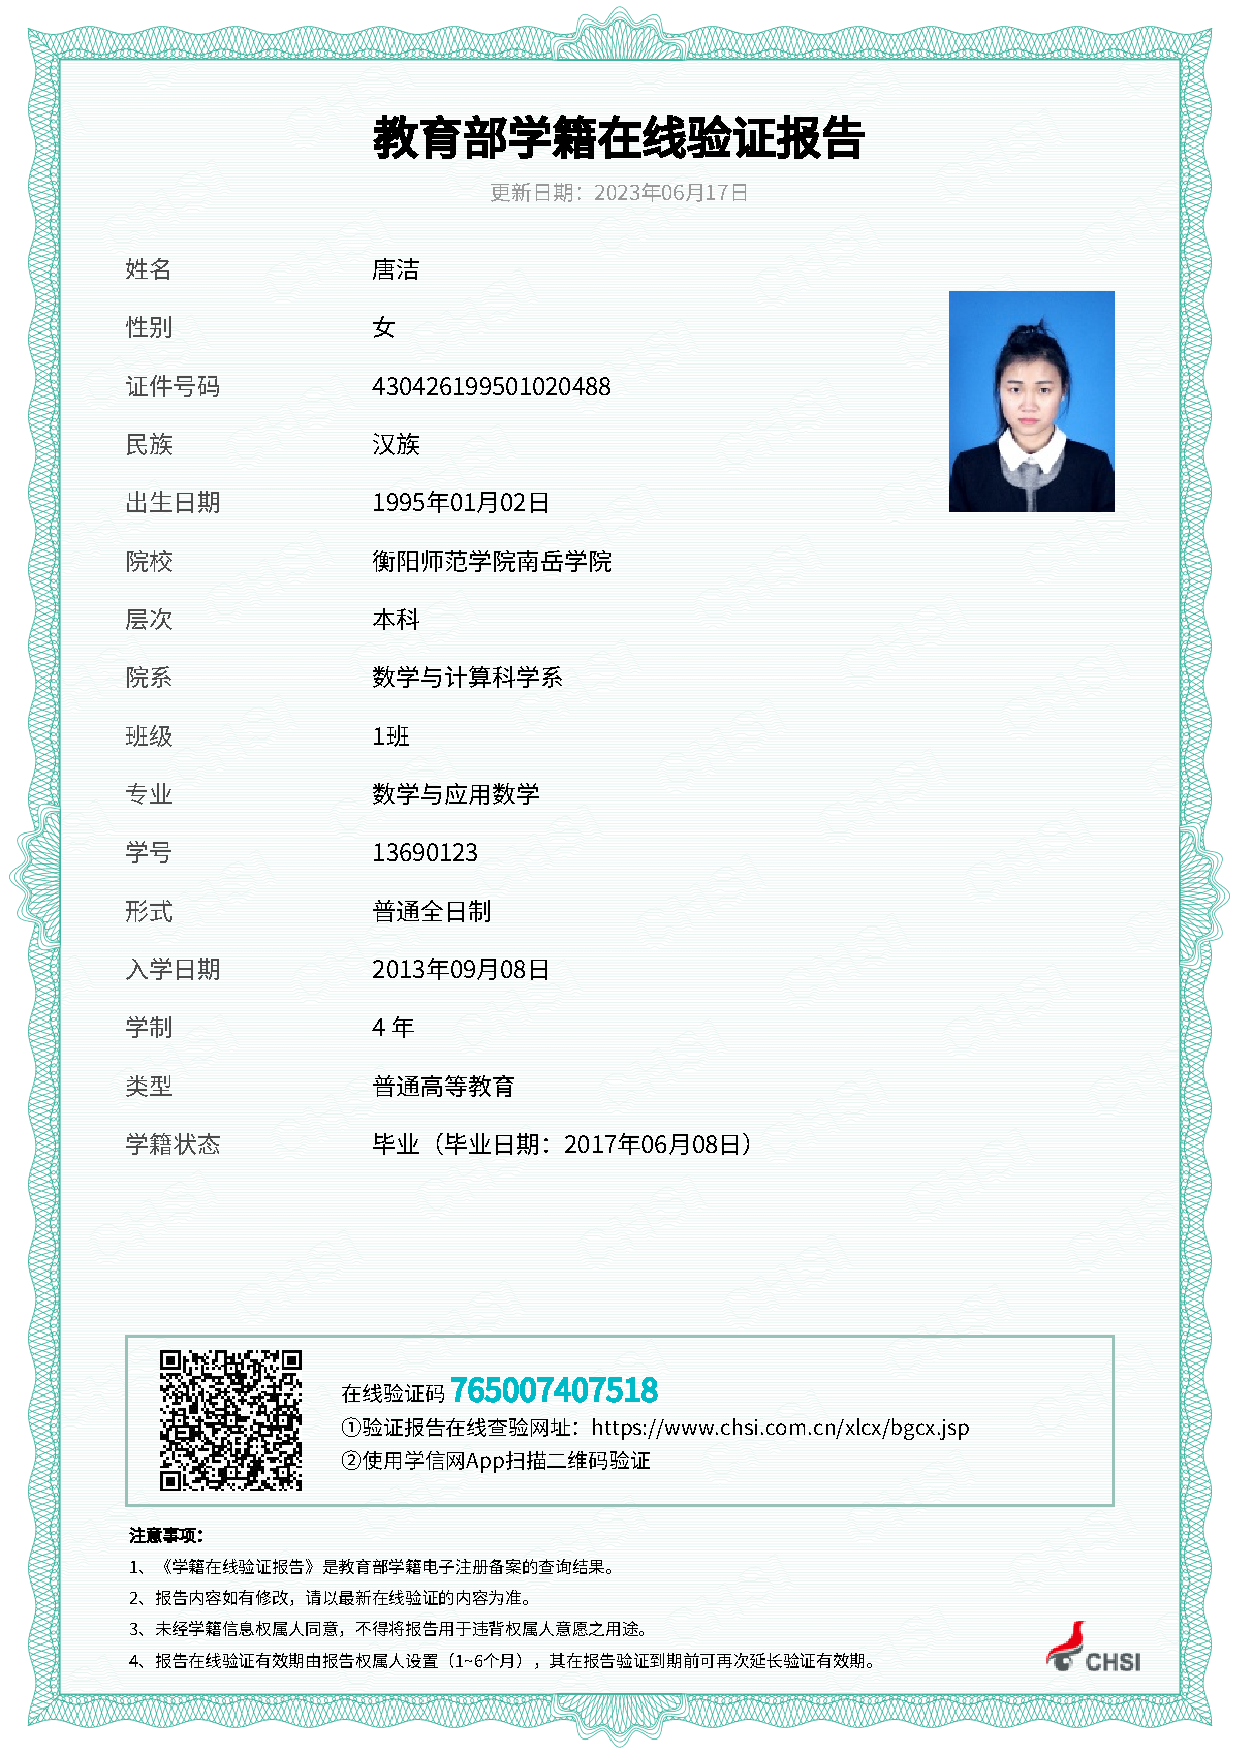
\includepdf[pages=1]{pdfs/教育部学籍在线验证报告本科.pdf}
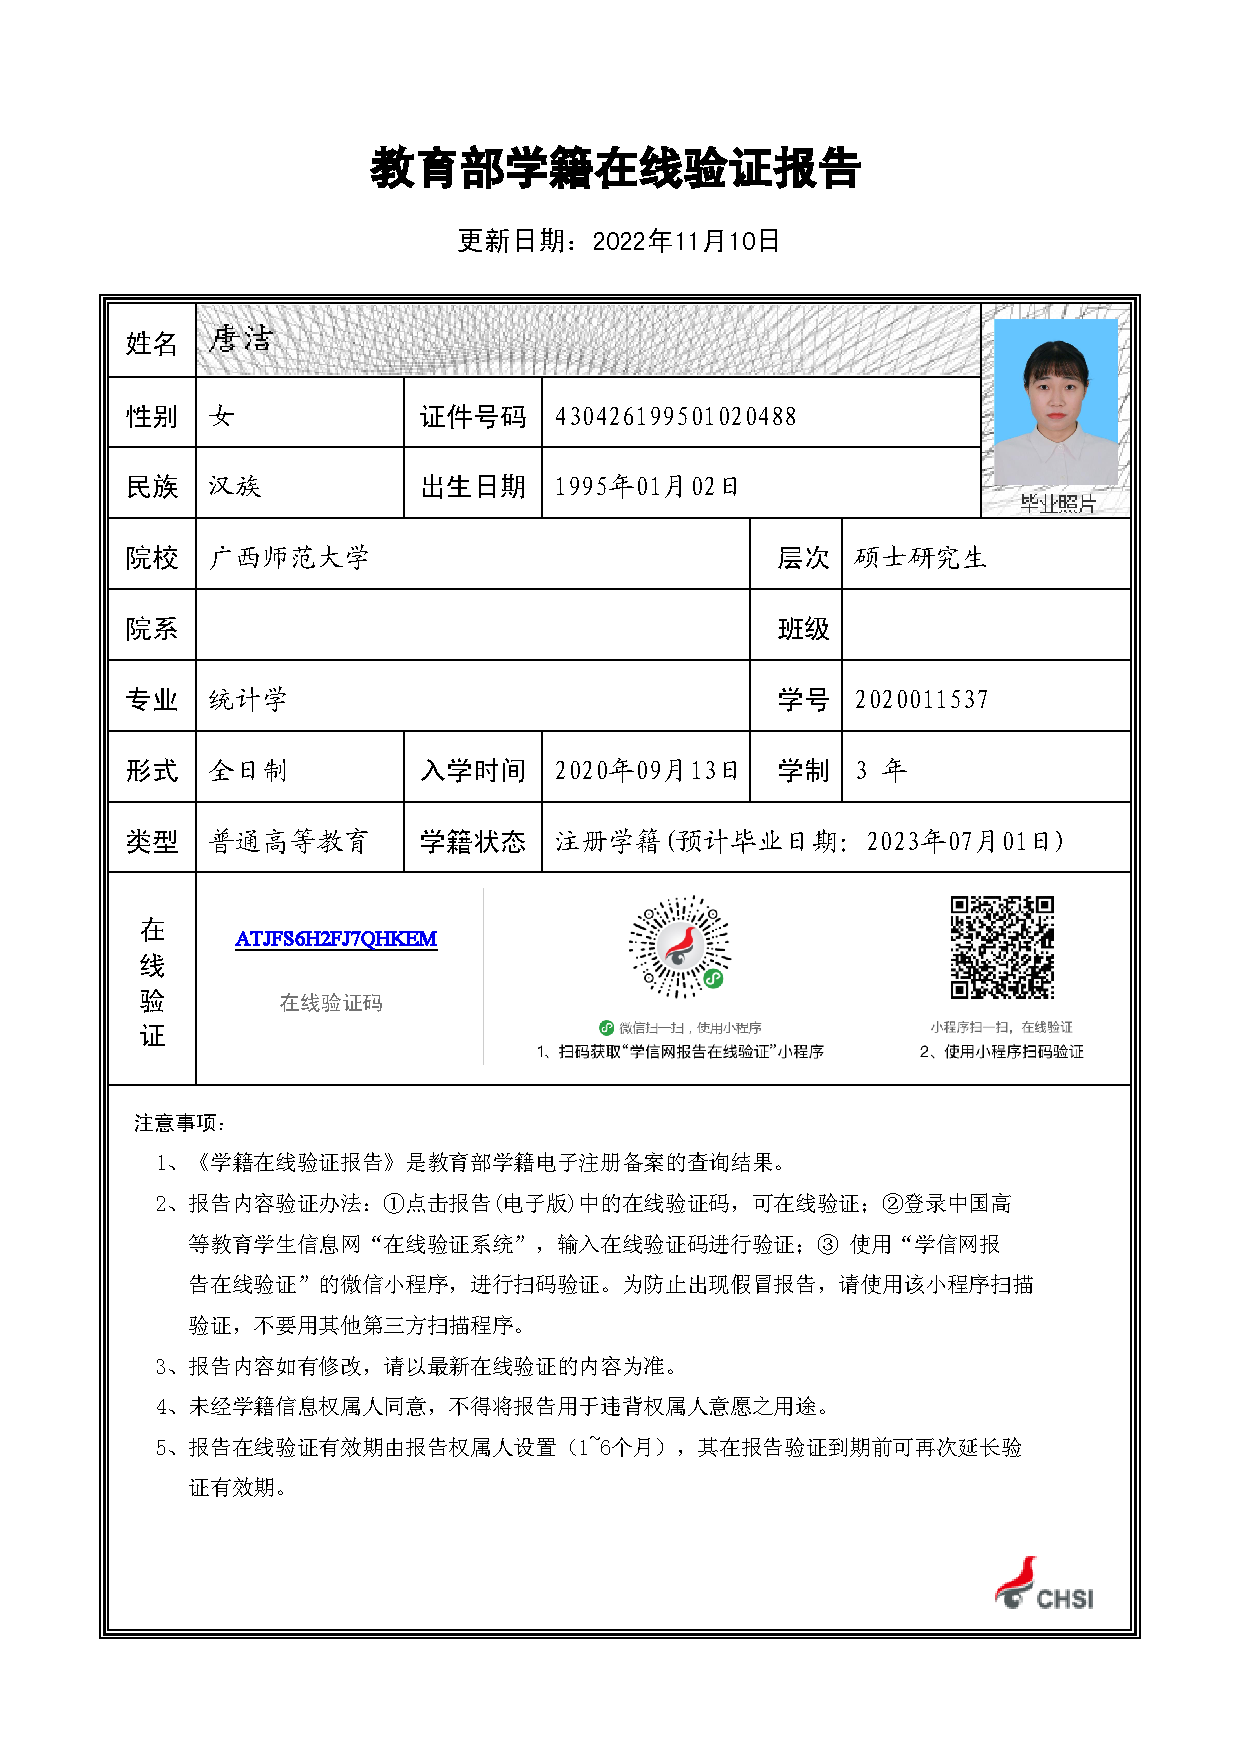
\includepdf[pages=1]{pdfs/教育部学籍在线验证报告硕士.pdf}

\clearpage

%\section{就业推荐表}
%\begin{center}
%  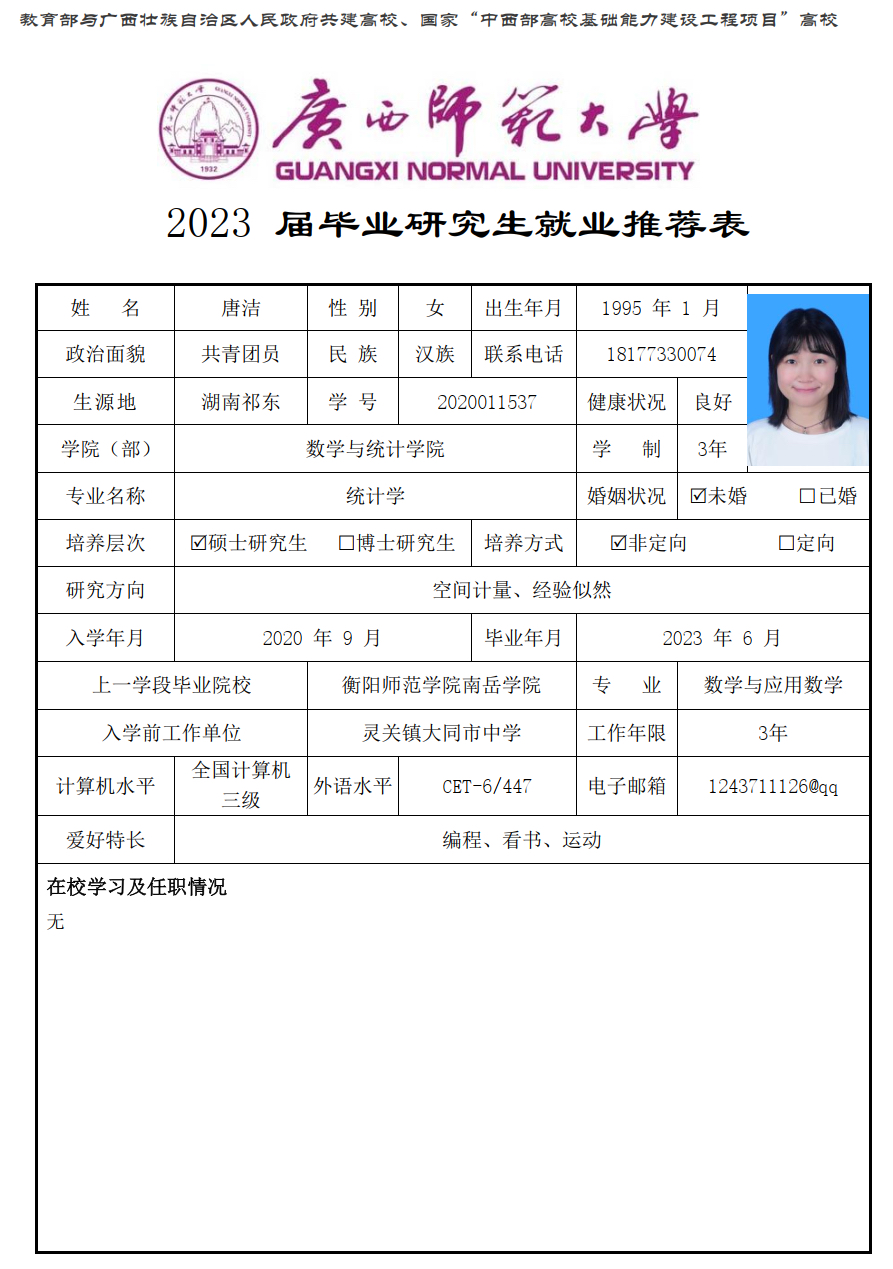
\includegraphics[scale=0.5]{figs/硕士就业推荐表1.JPG }
%  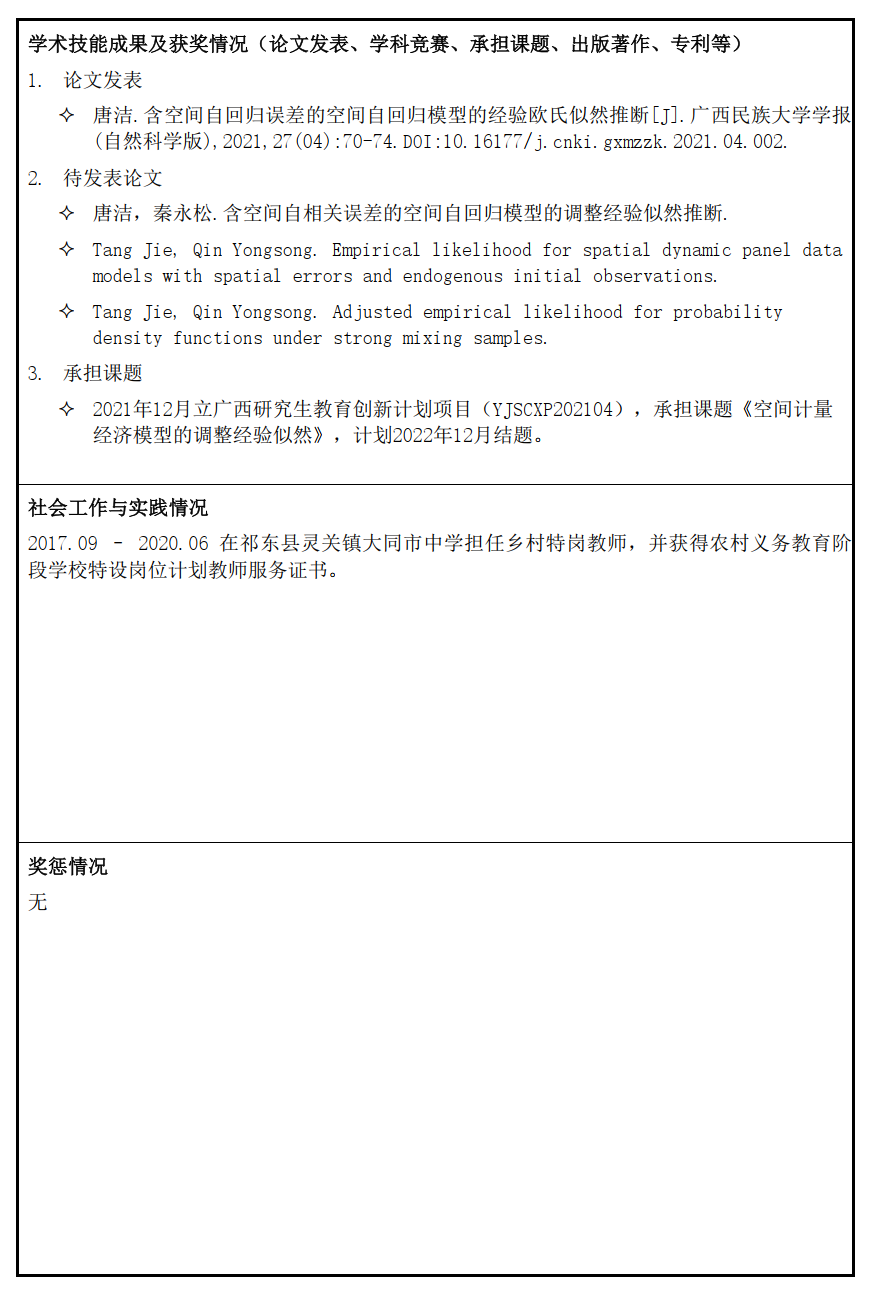
\includegraphics[scale=0.5]{figs/硕士就业推荐表3.JPG }
%  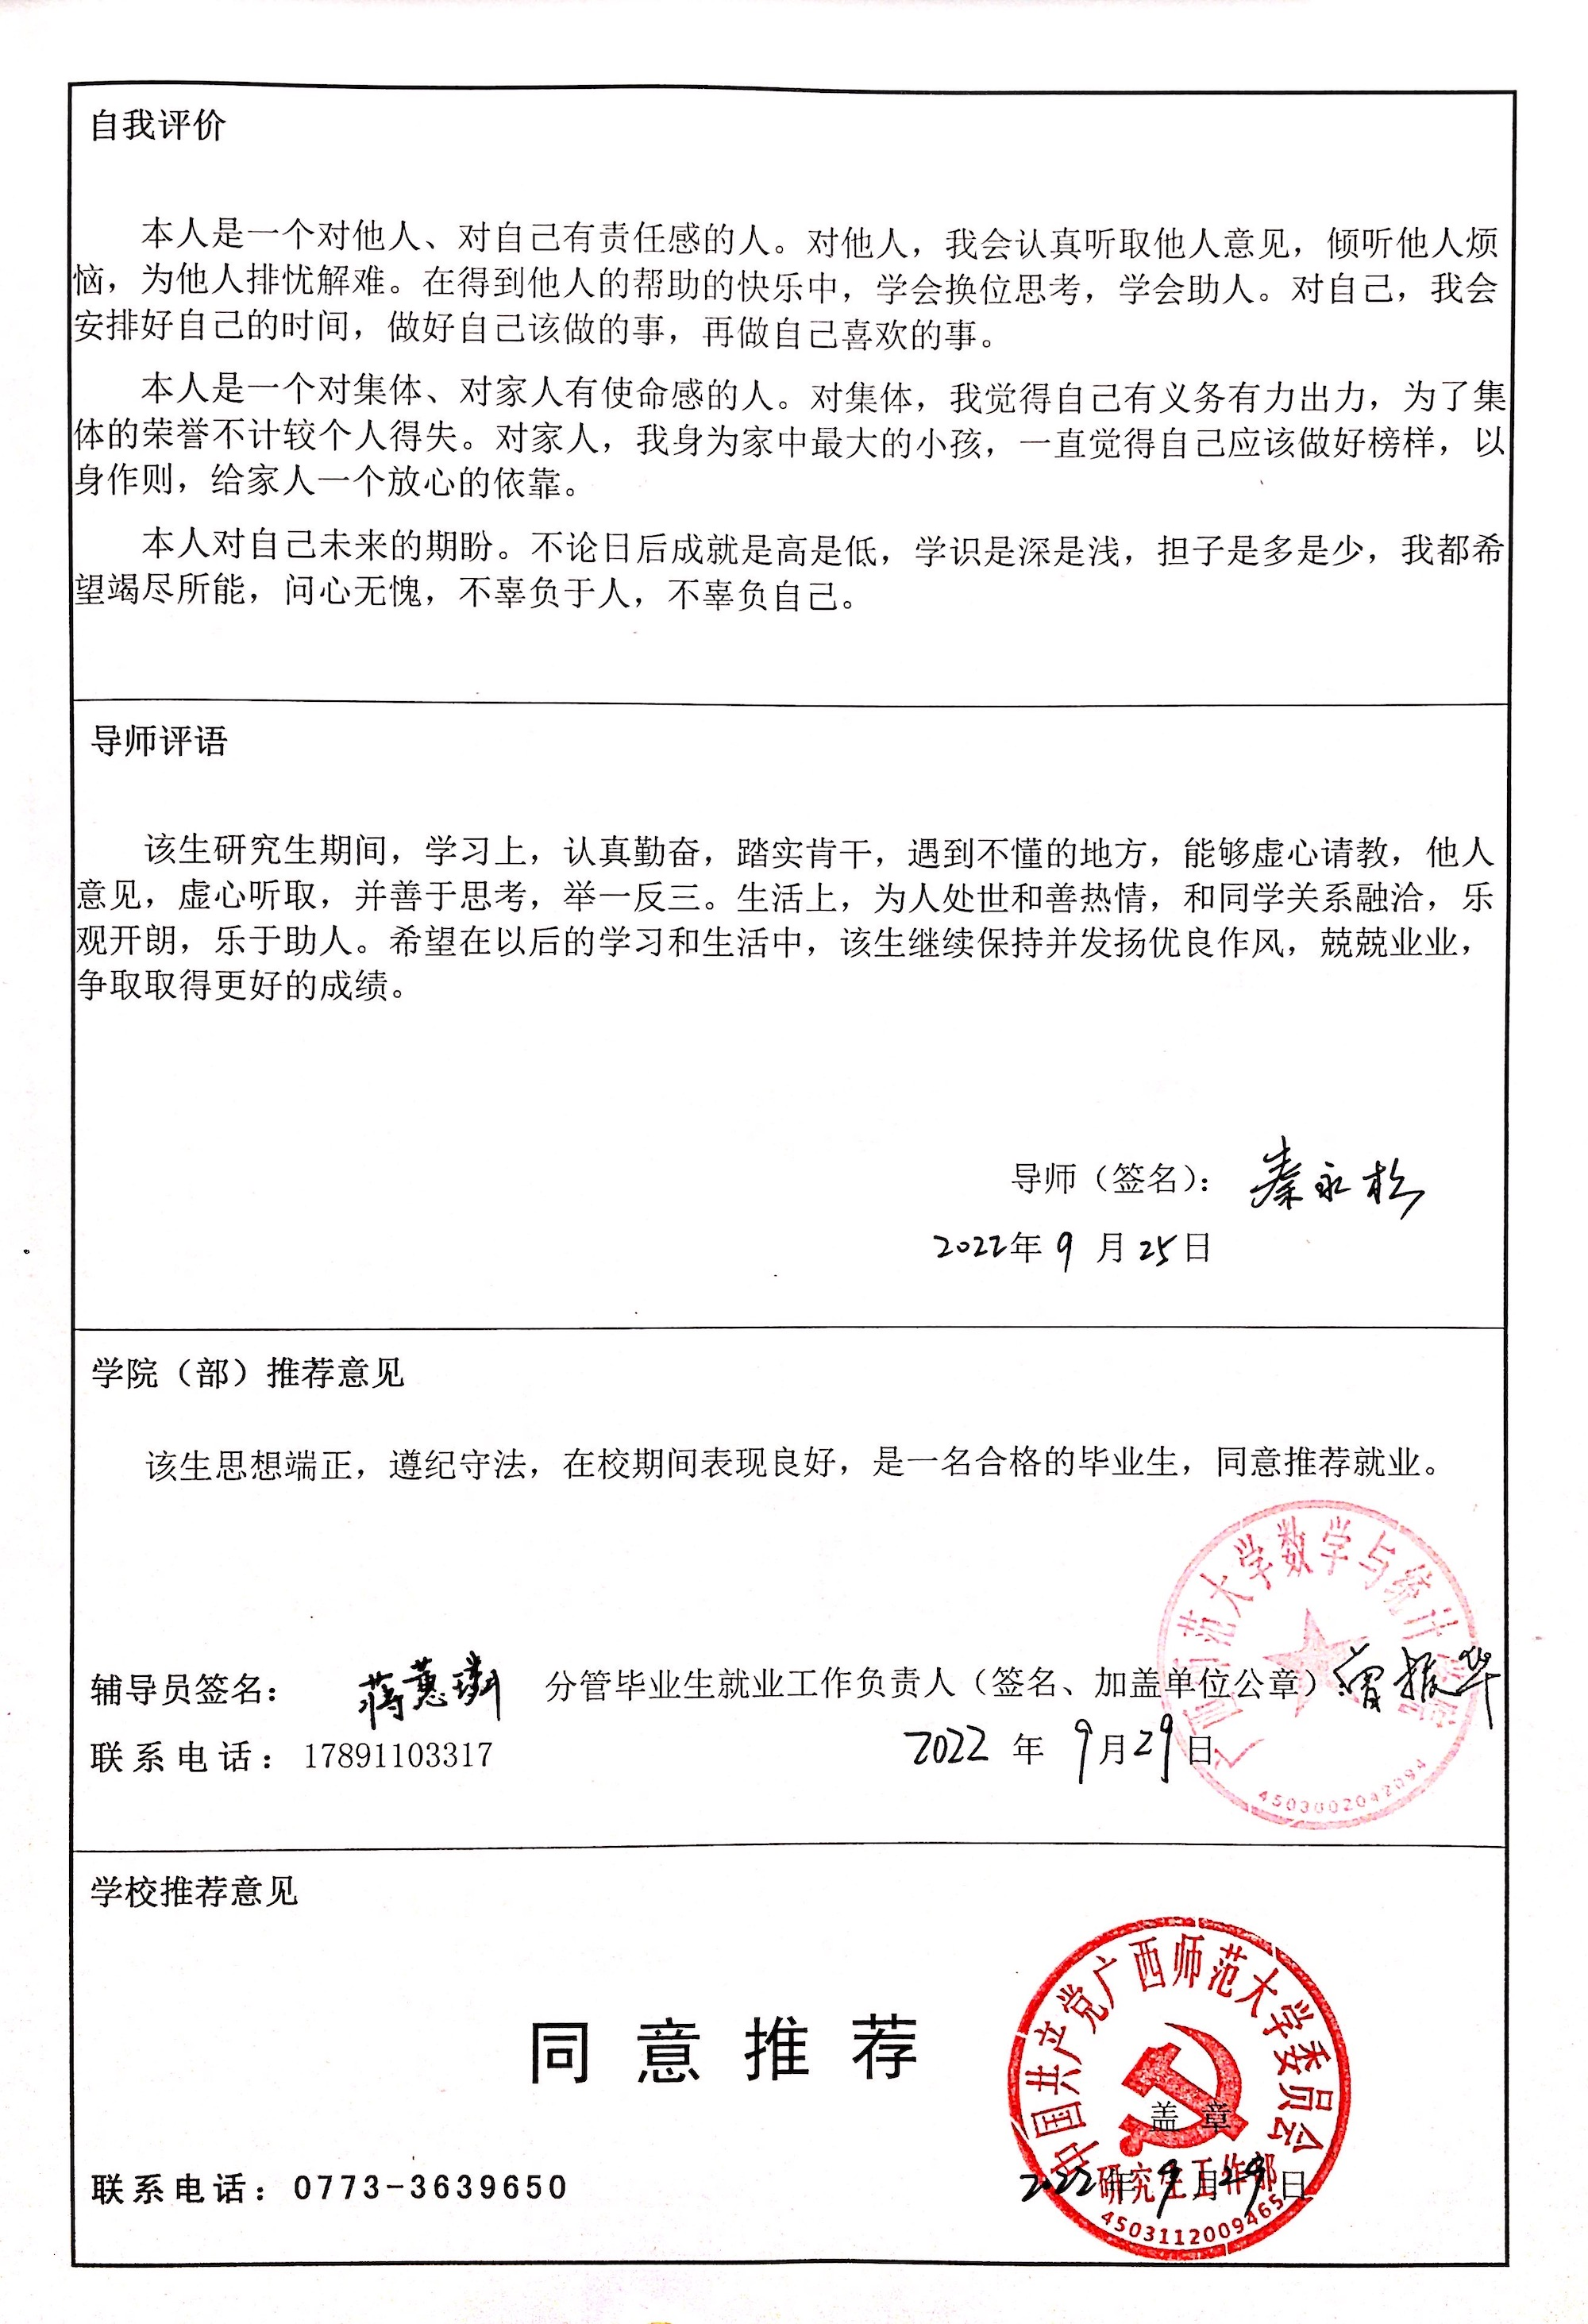
\includegraphics[scale=0.37]{figs/硕士就业推荐表4.JPG }
%\end{center}



%\section{成绩单}
%\begin{center}
%
% 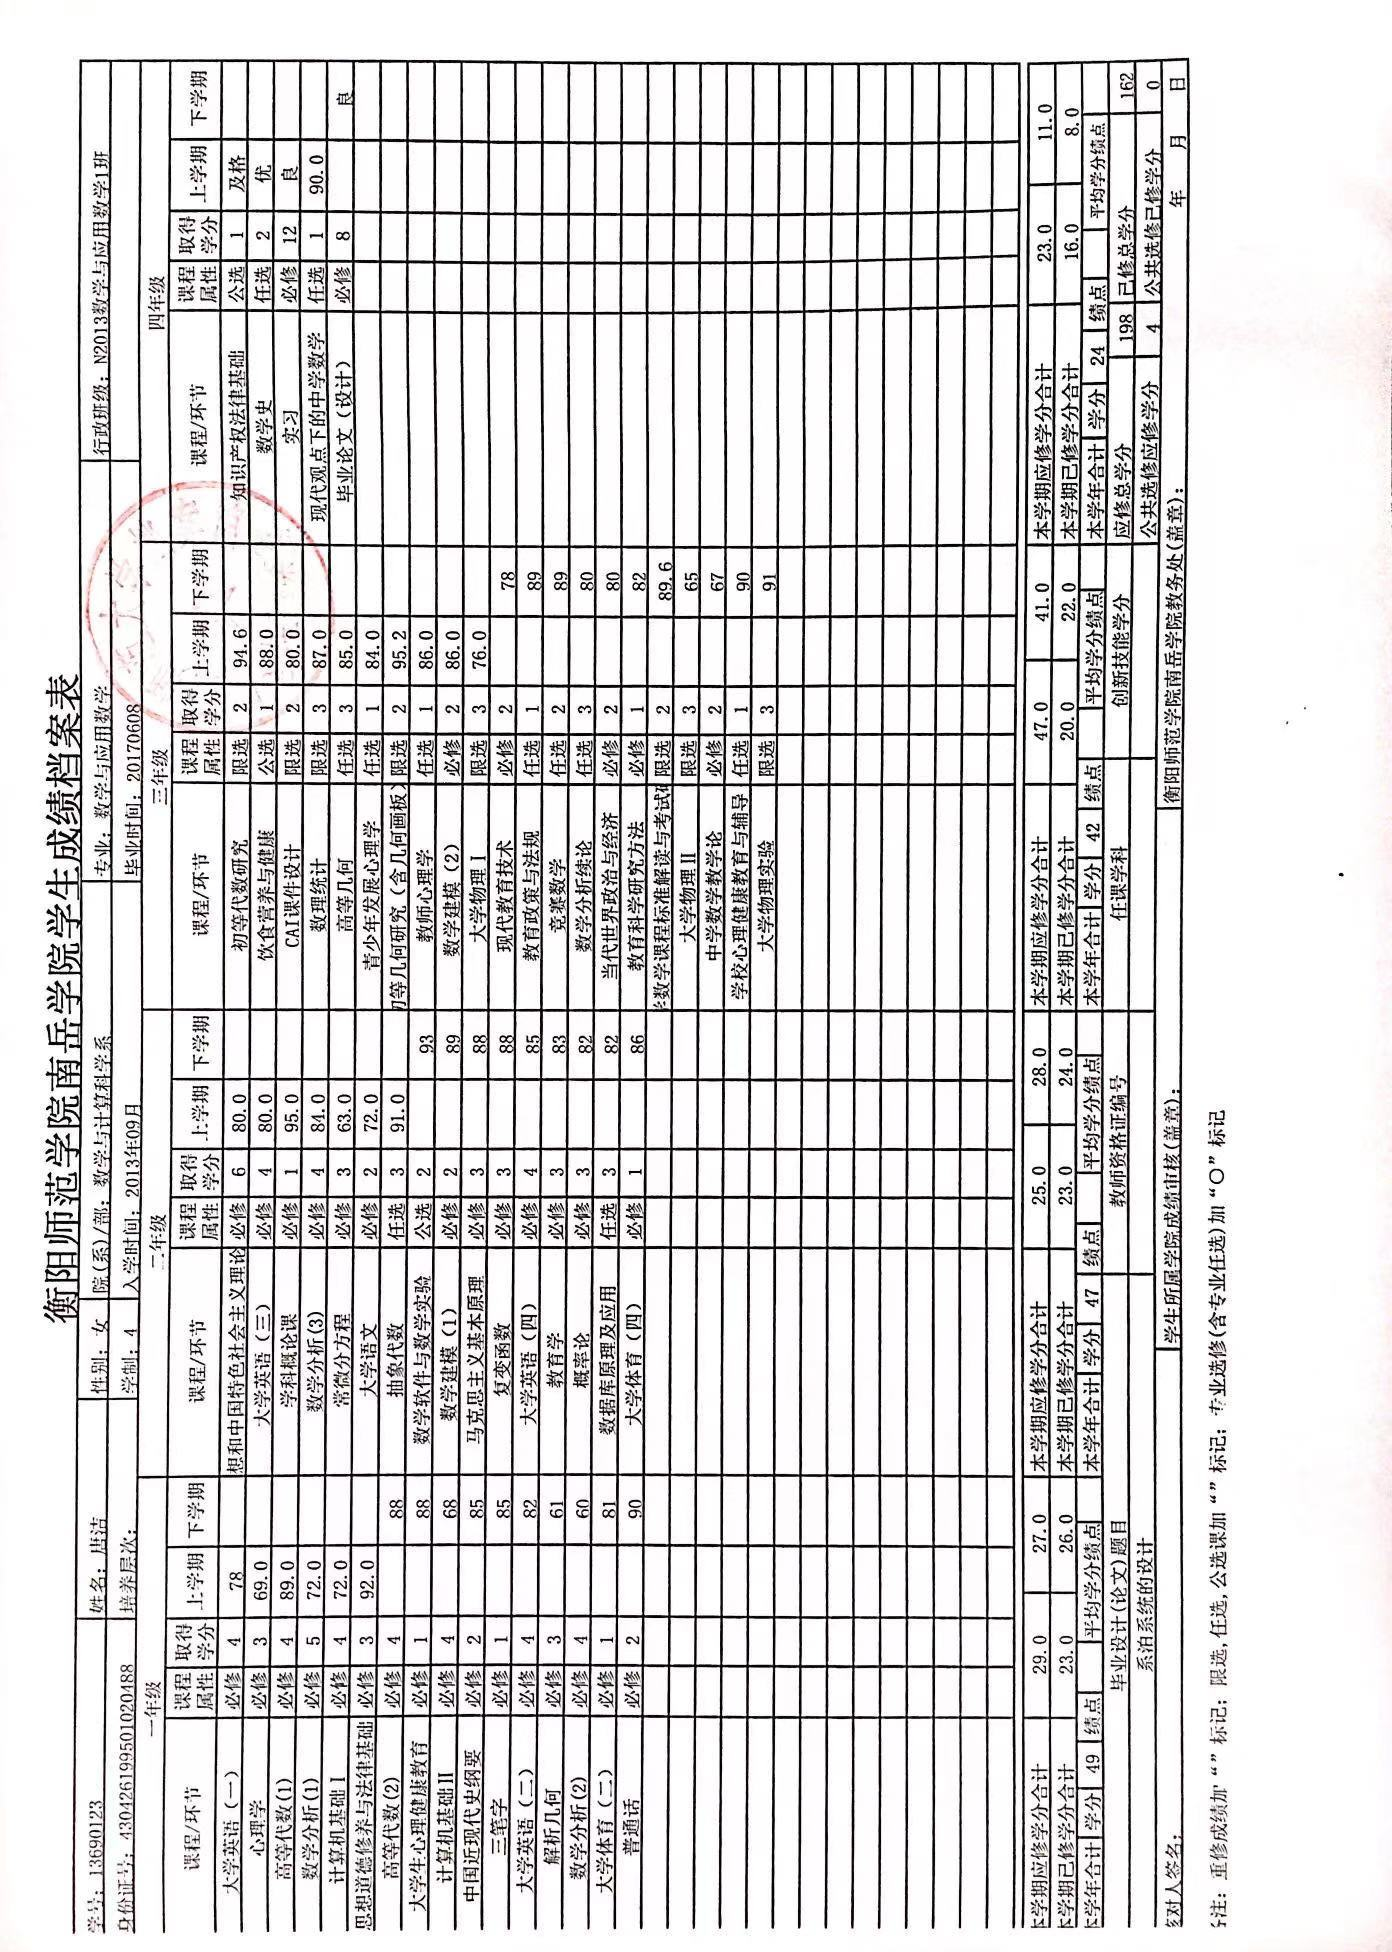
\includegraphics[scale=0.28]{figs/本科成绩单.JPG }
%
%  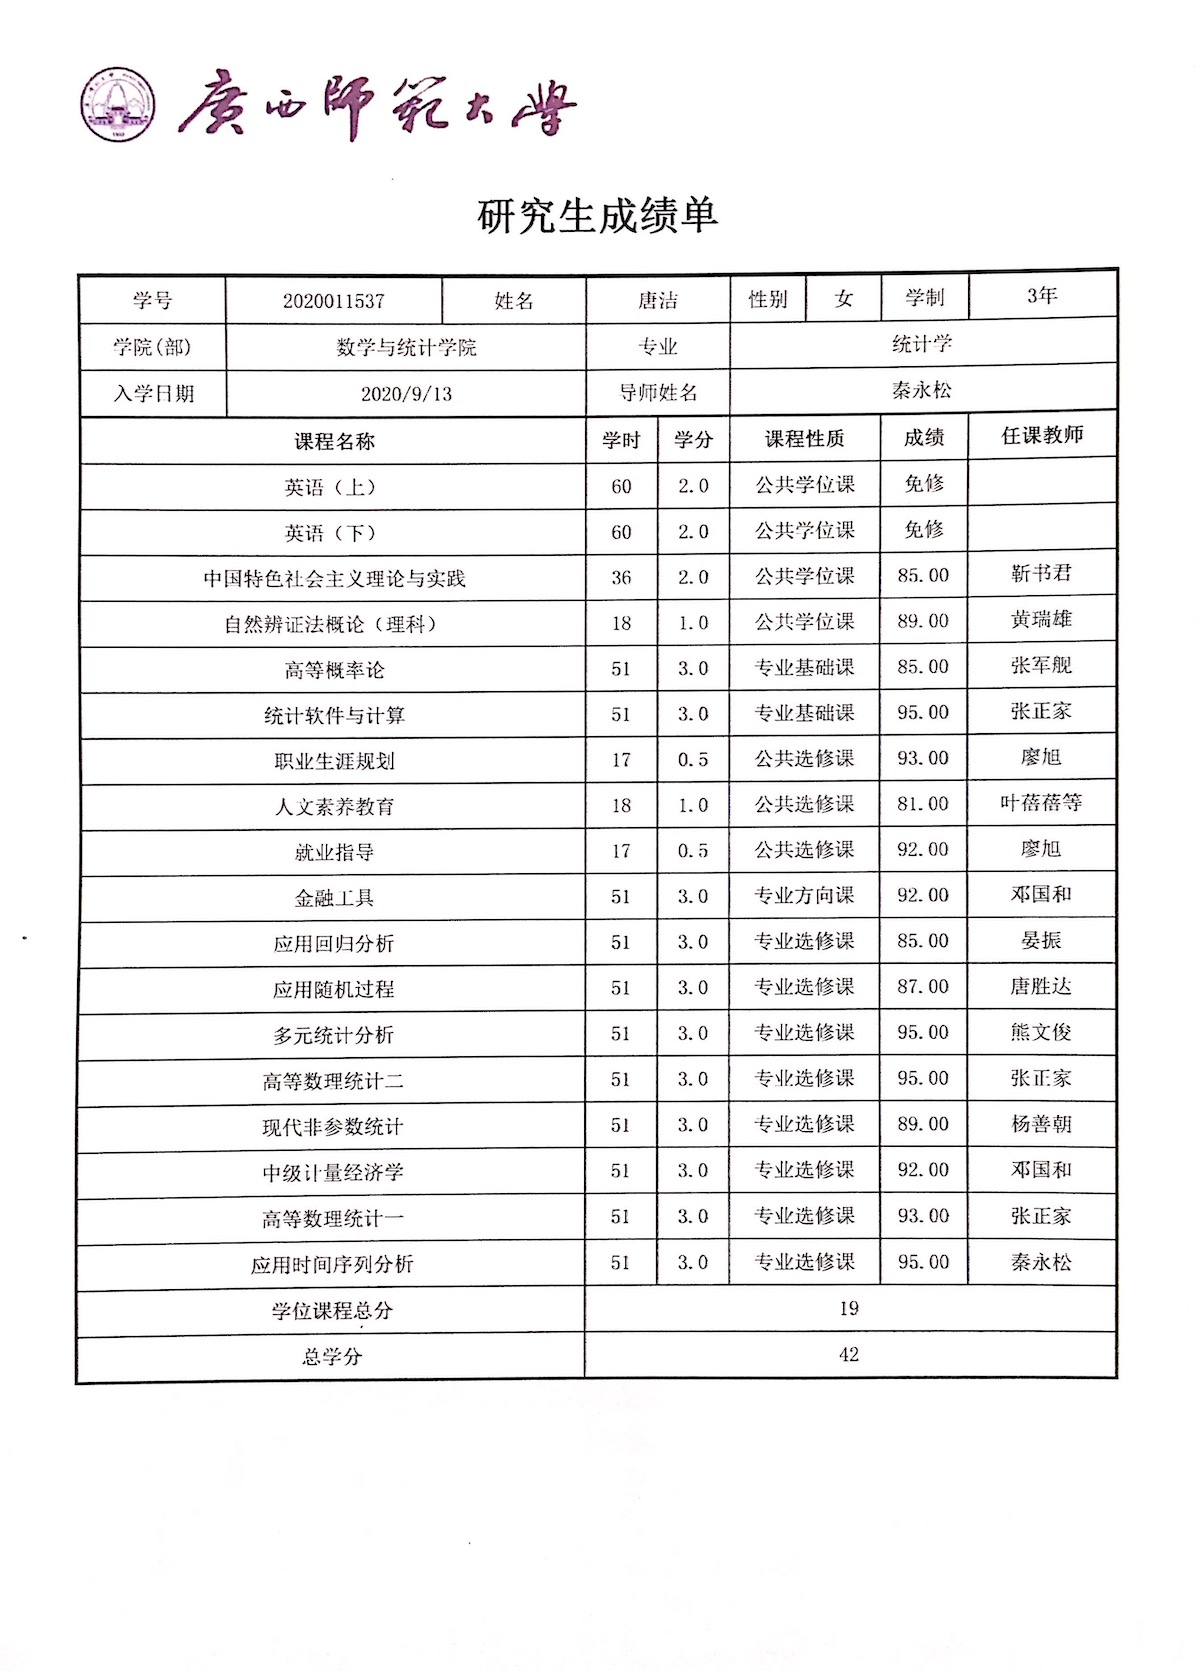
\includegraphics[scale=0.4]{figs/硕士成绩单1.JPG }
%  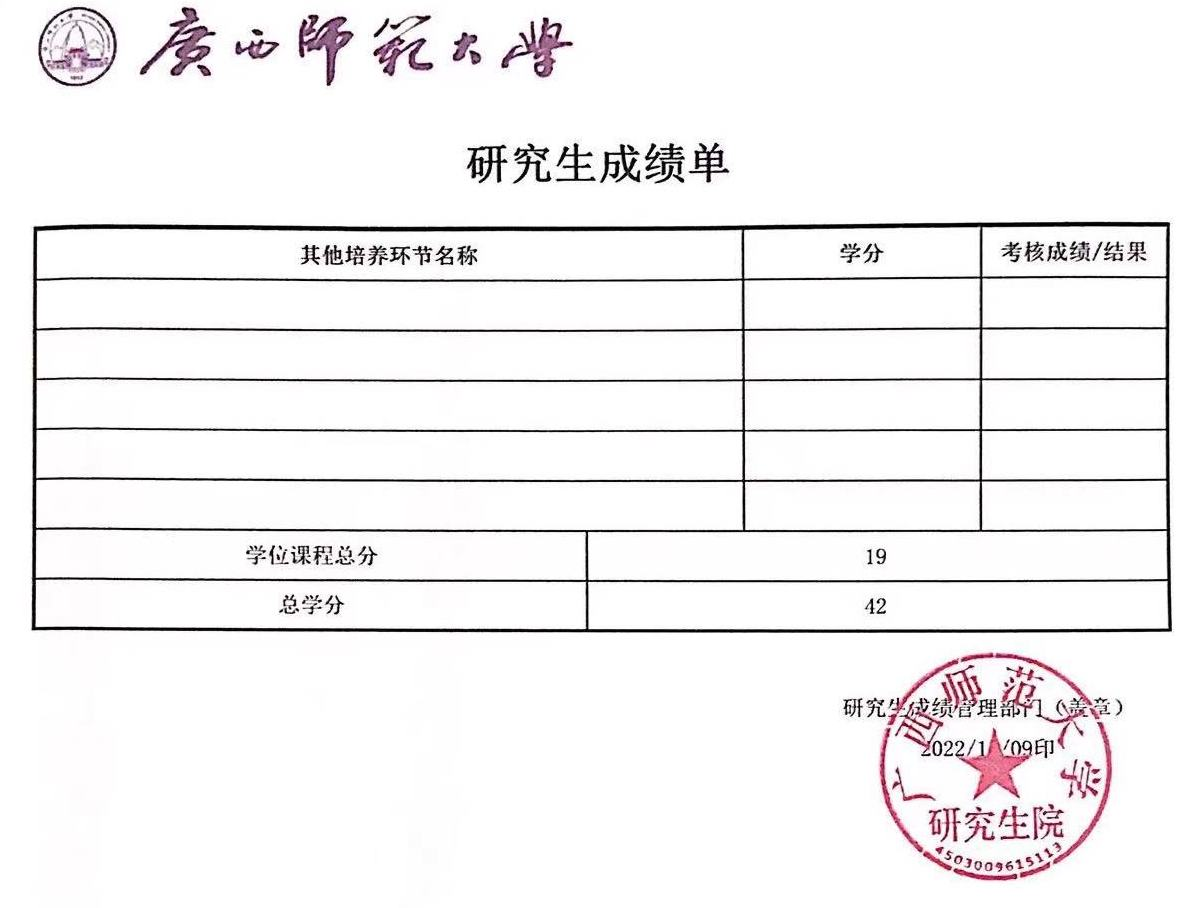
\includegraphics[scale=0.35]{figs/硕士成绩单2.JPG }
%\end{center}

\clearpage
\section{相关证件}
\begin{center}
教师资格证
  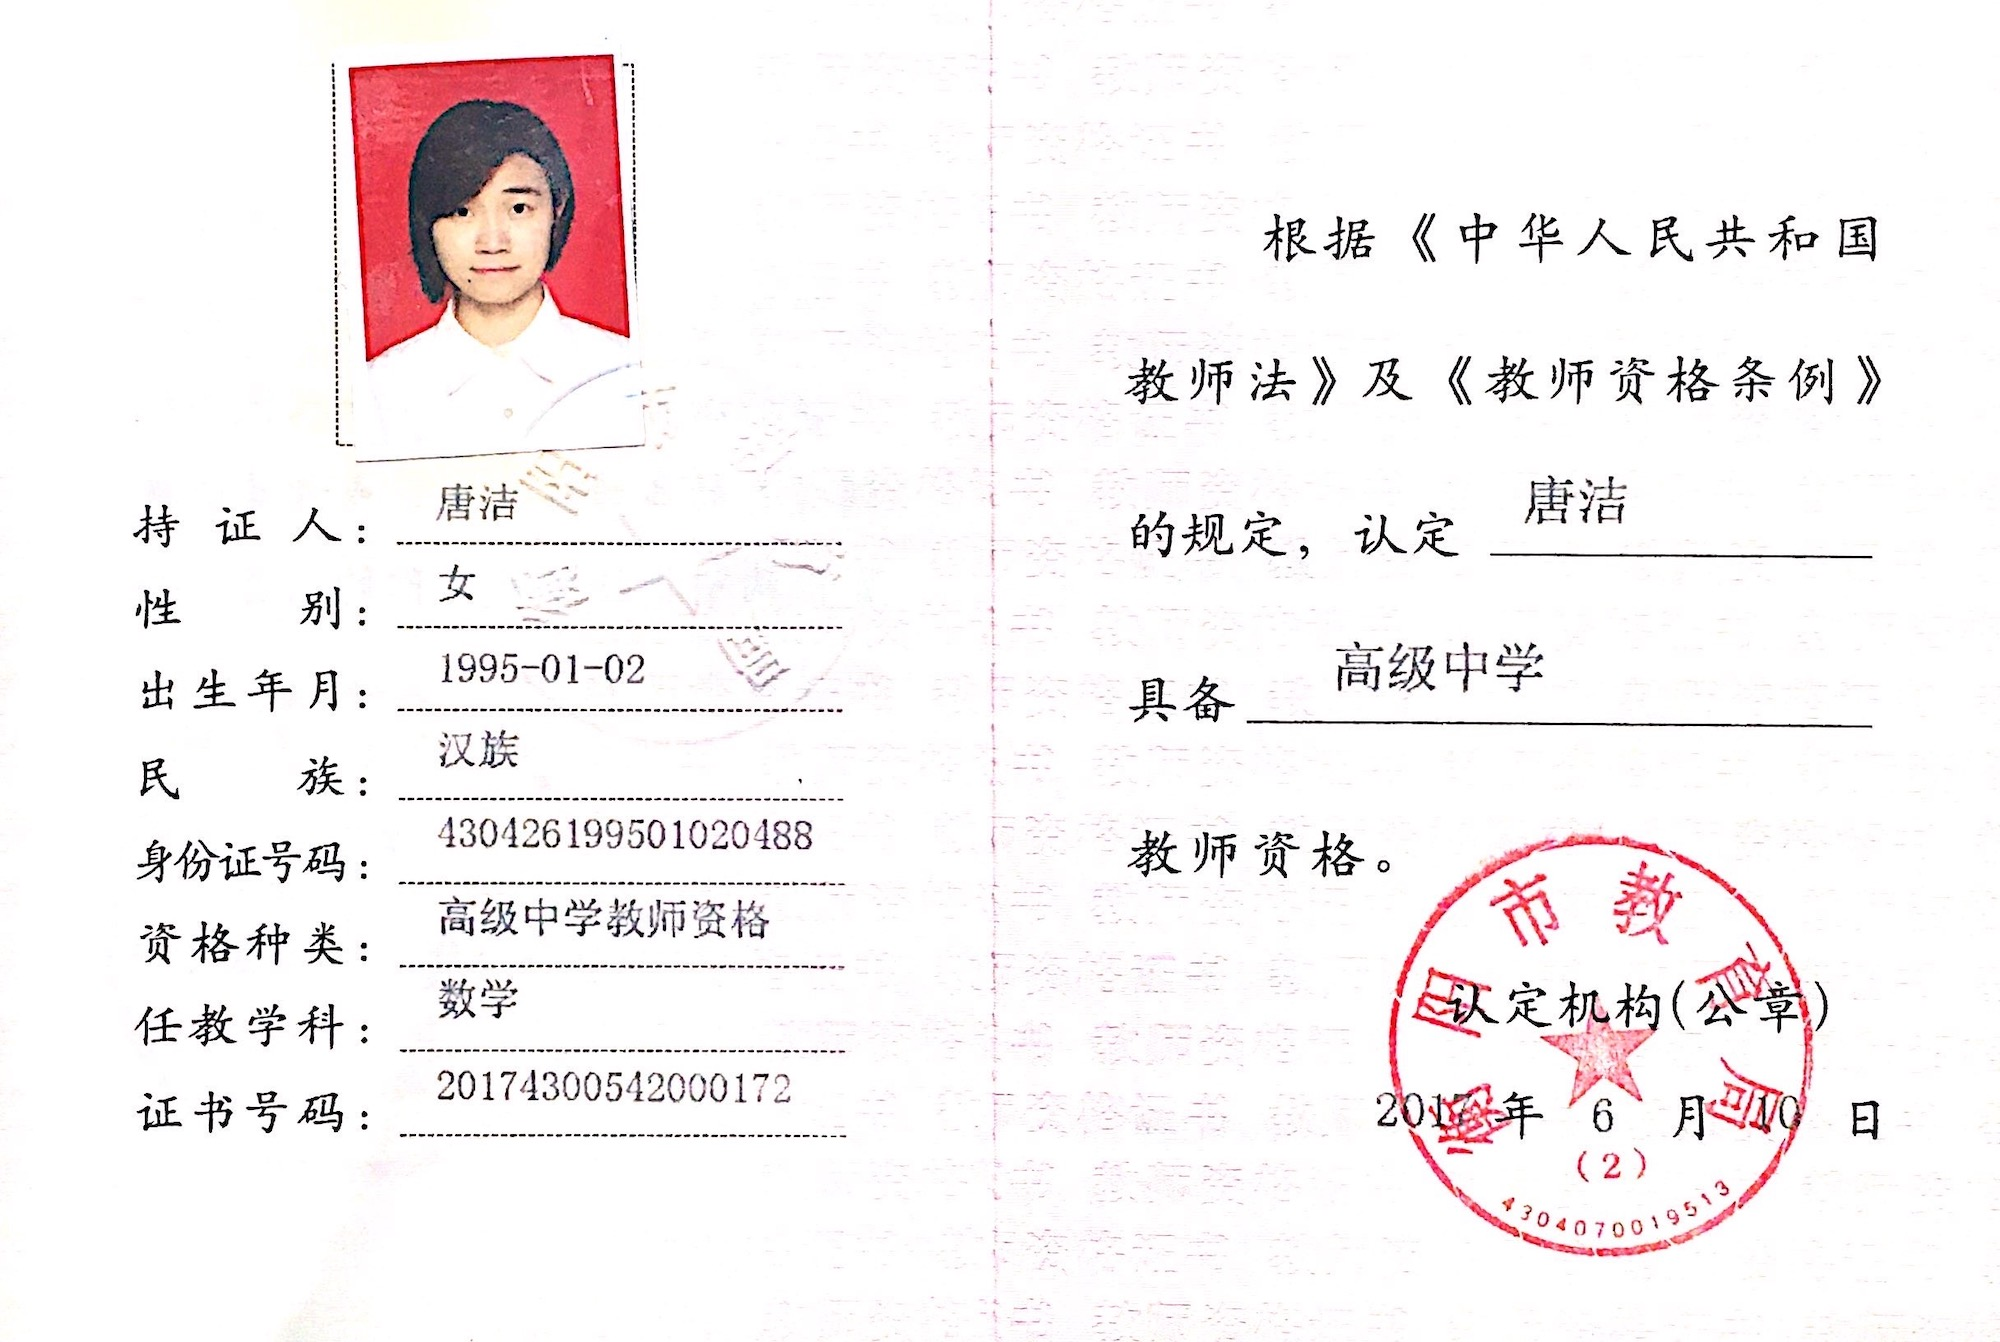
\includegraphics[scale=0.20]{figs/教师资格证.JPG }

职称证书
  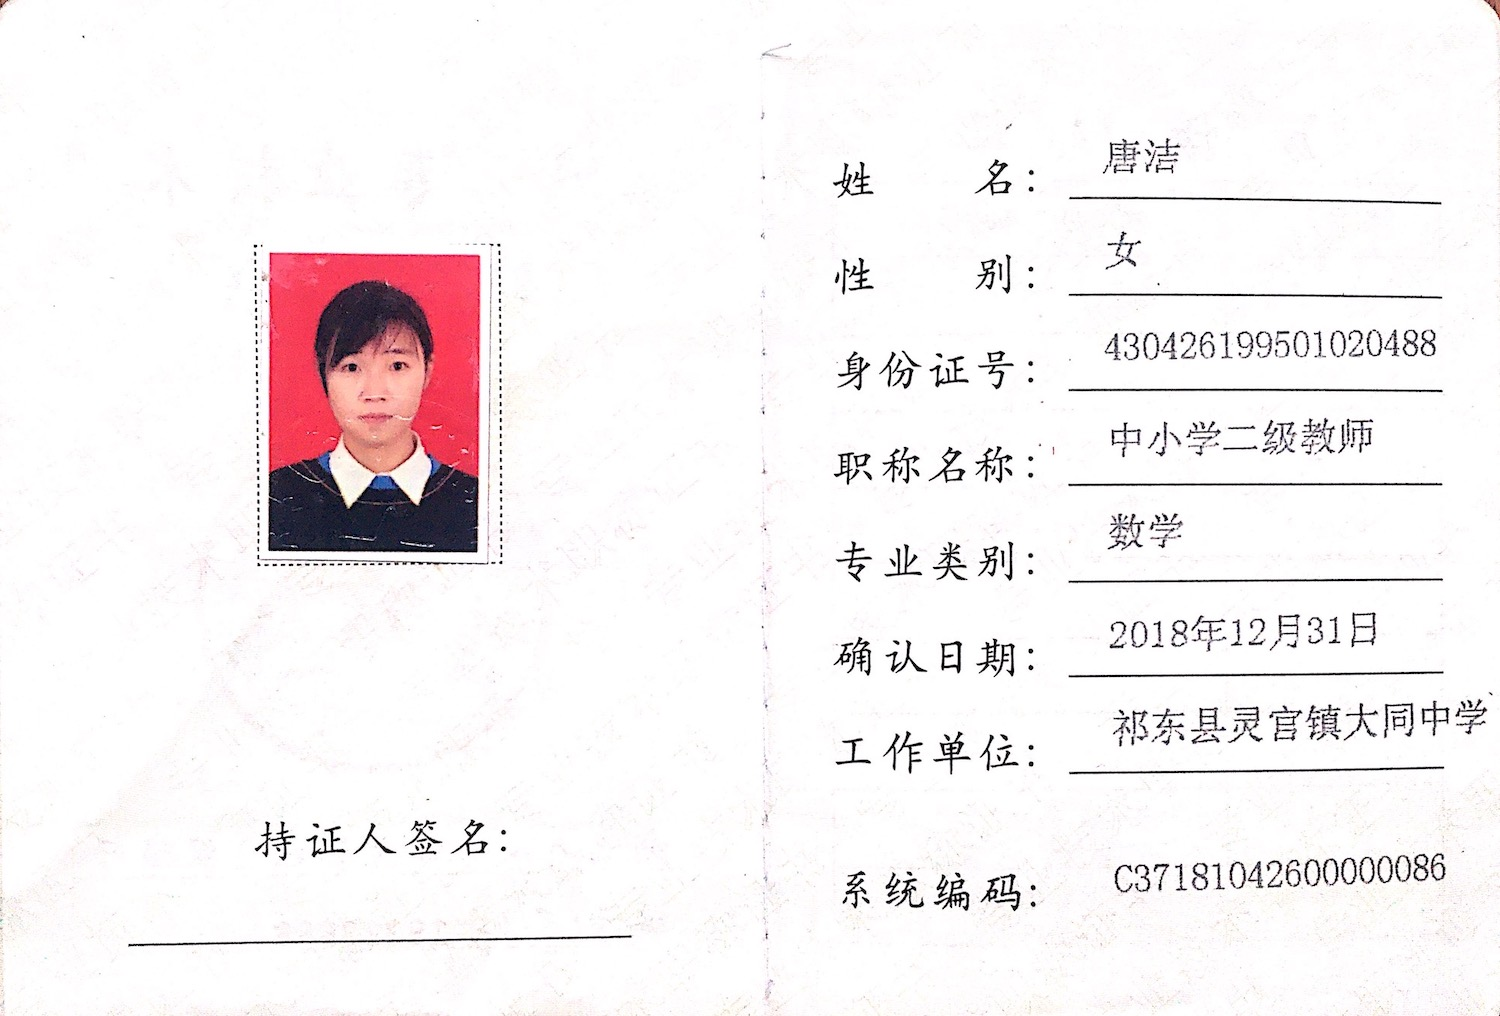
\includegraphics[scale=0.25]{figs/中二职称证书.JPG }
  
计算机二级证
  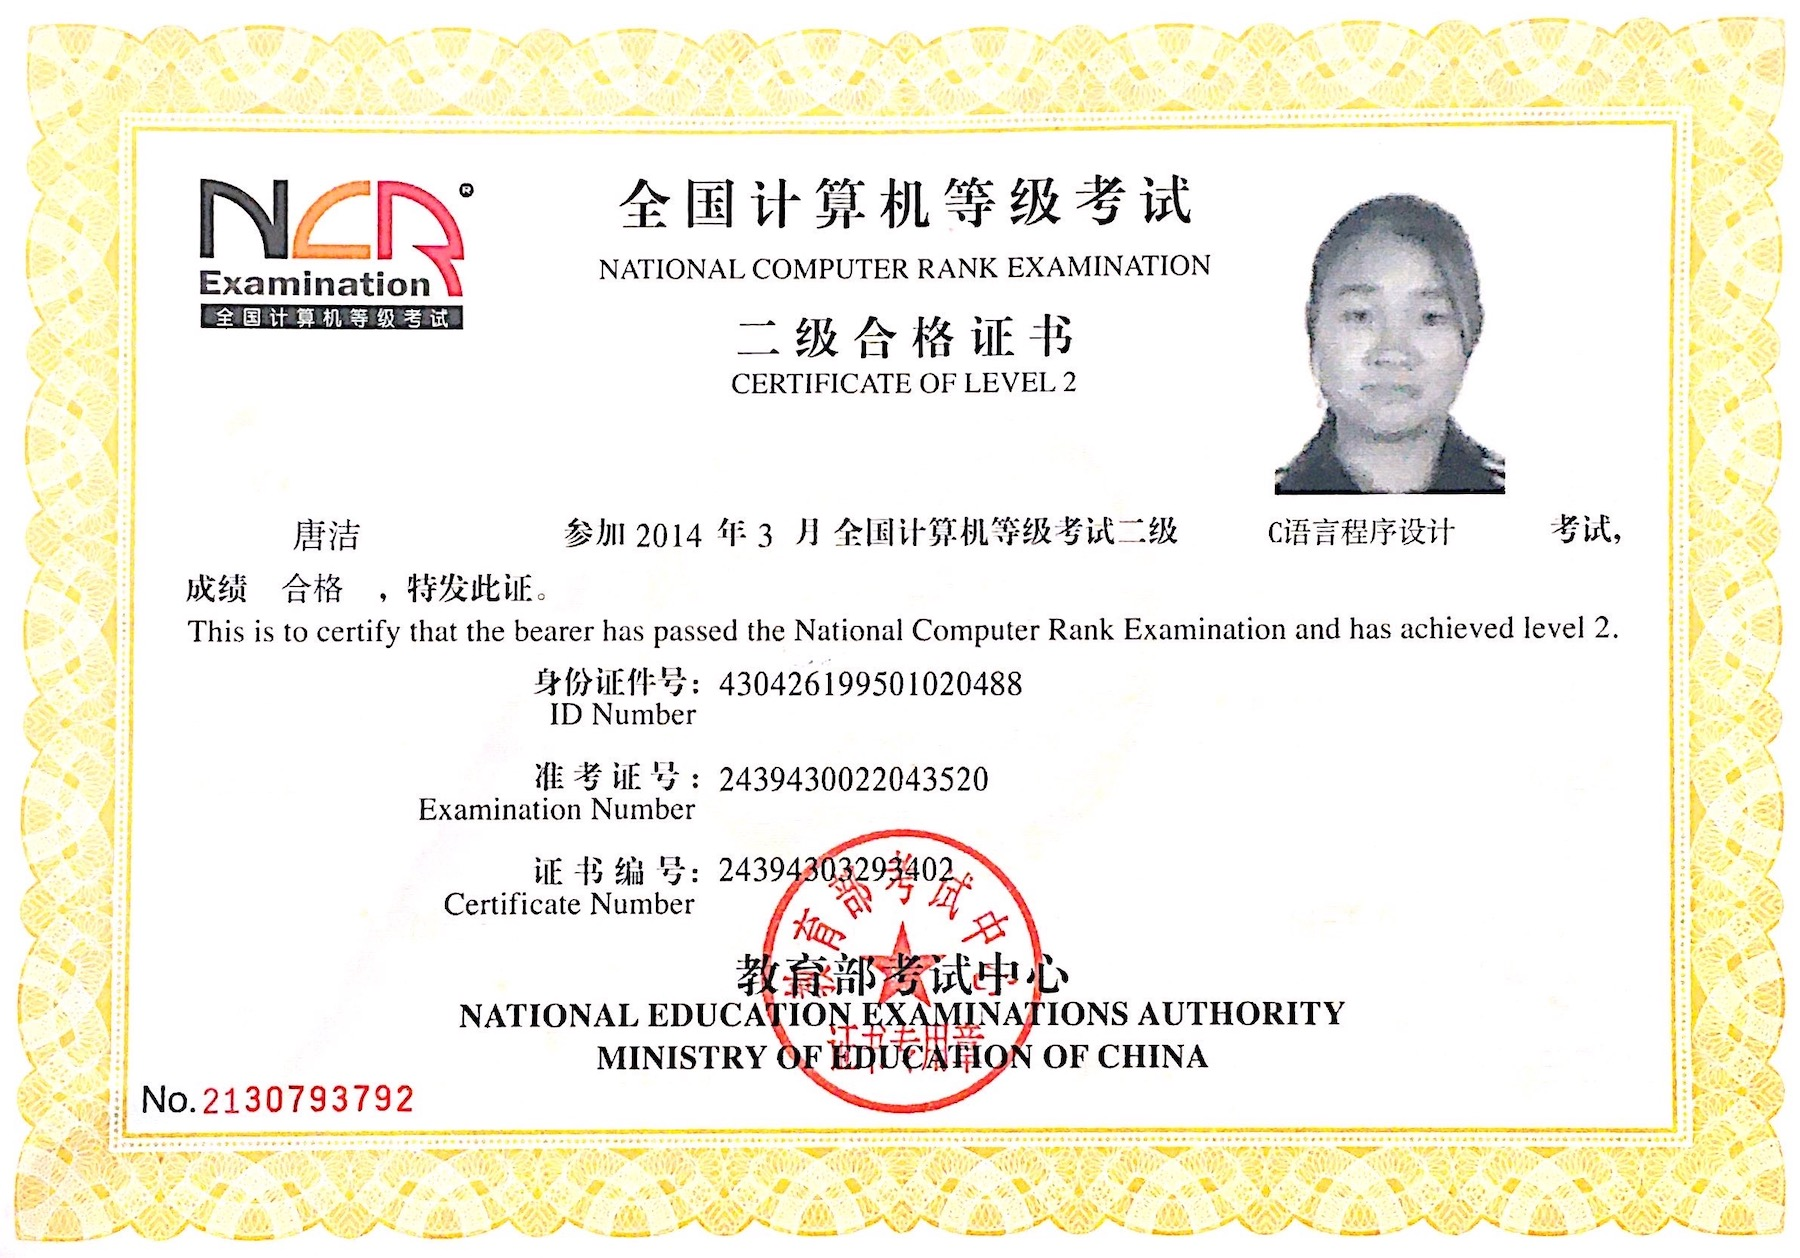
\includegraphics[scale=0.22]{figs/计算机二级C.JPG }
  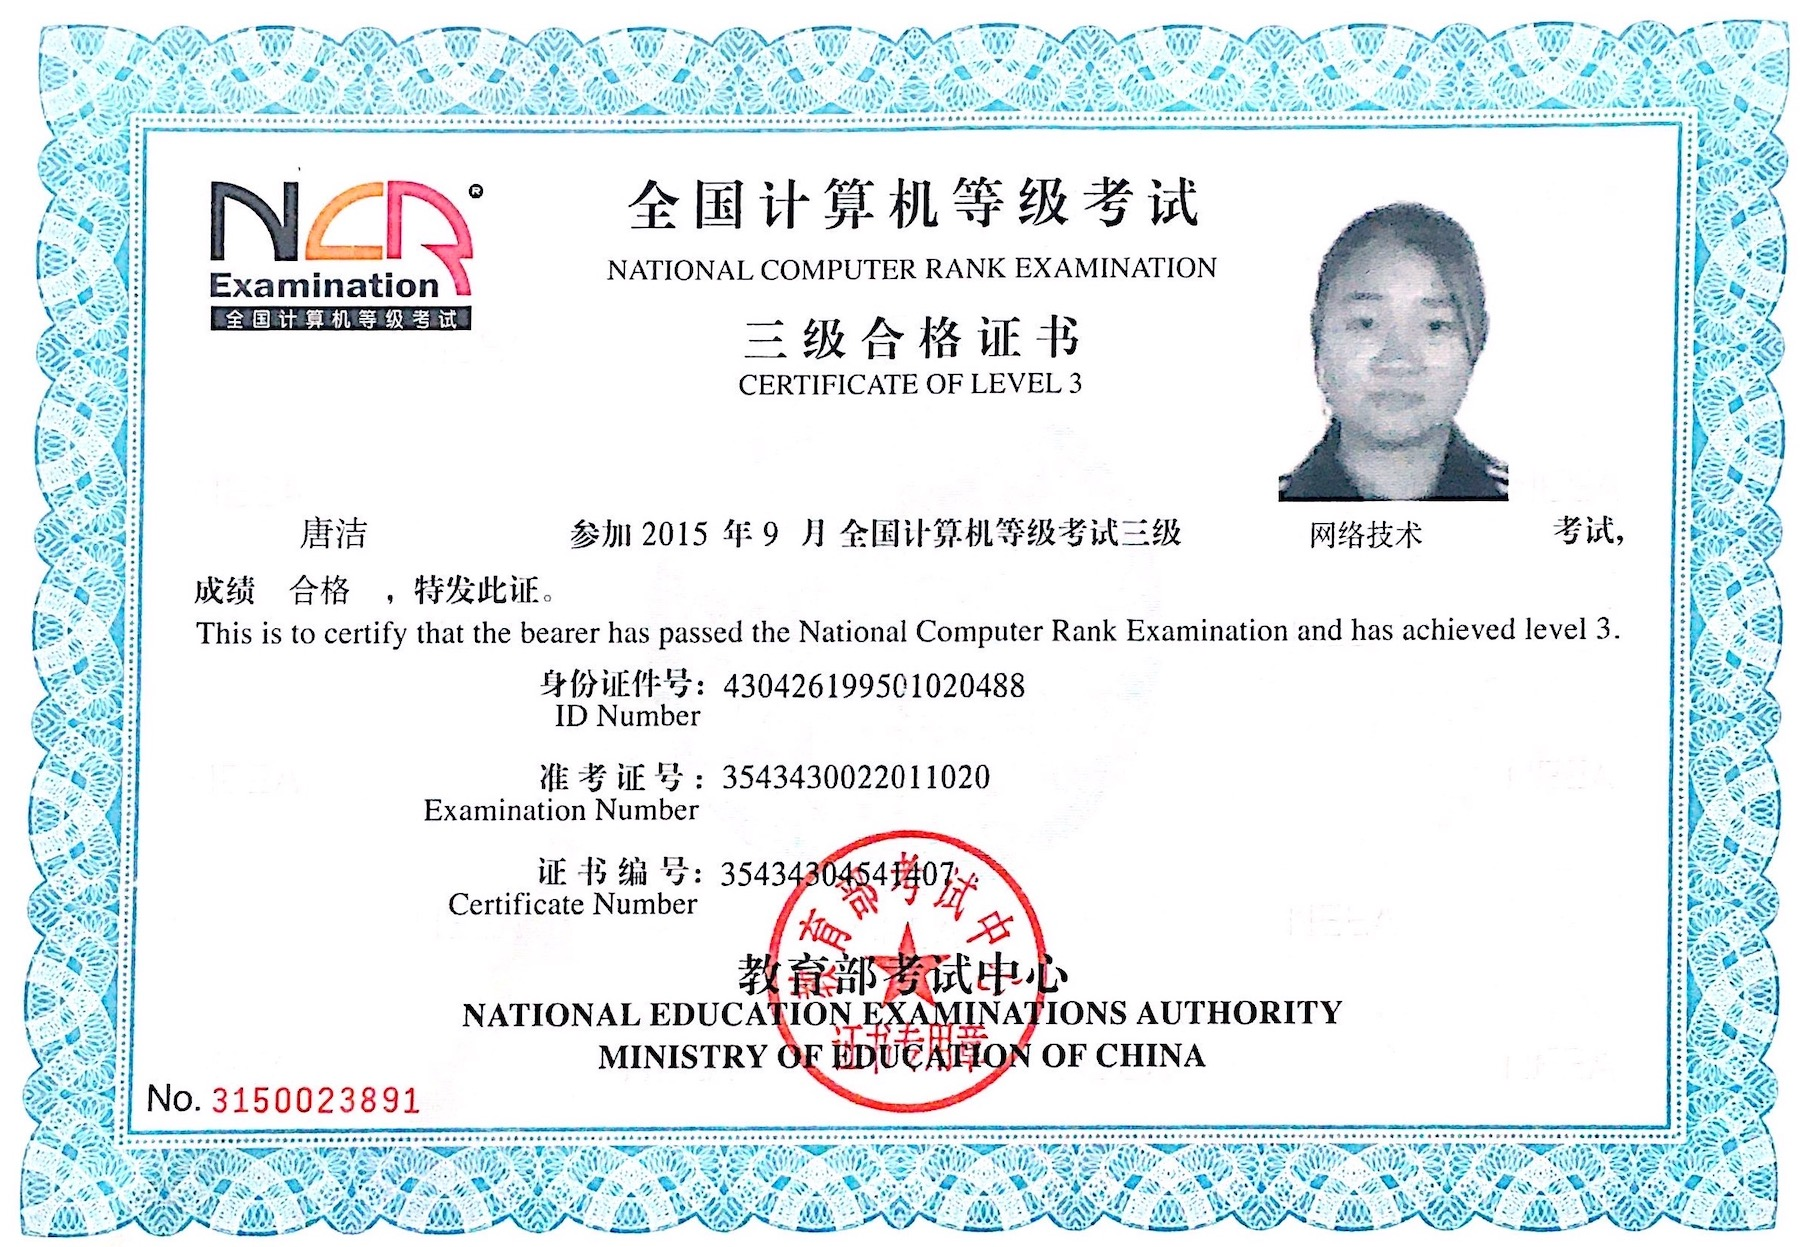
\includegraphics[scale=0.22]{figs/计算机三级证书.JPG }
   
计算机三级证
   
\includegraphics[scale=0.45]{figs/计算机二级Python.JPG }

普通话证
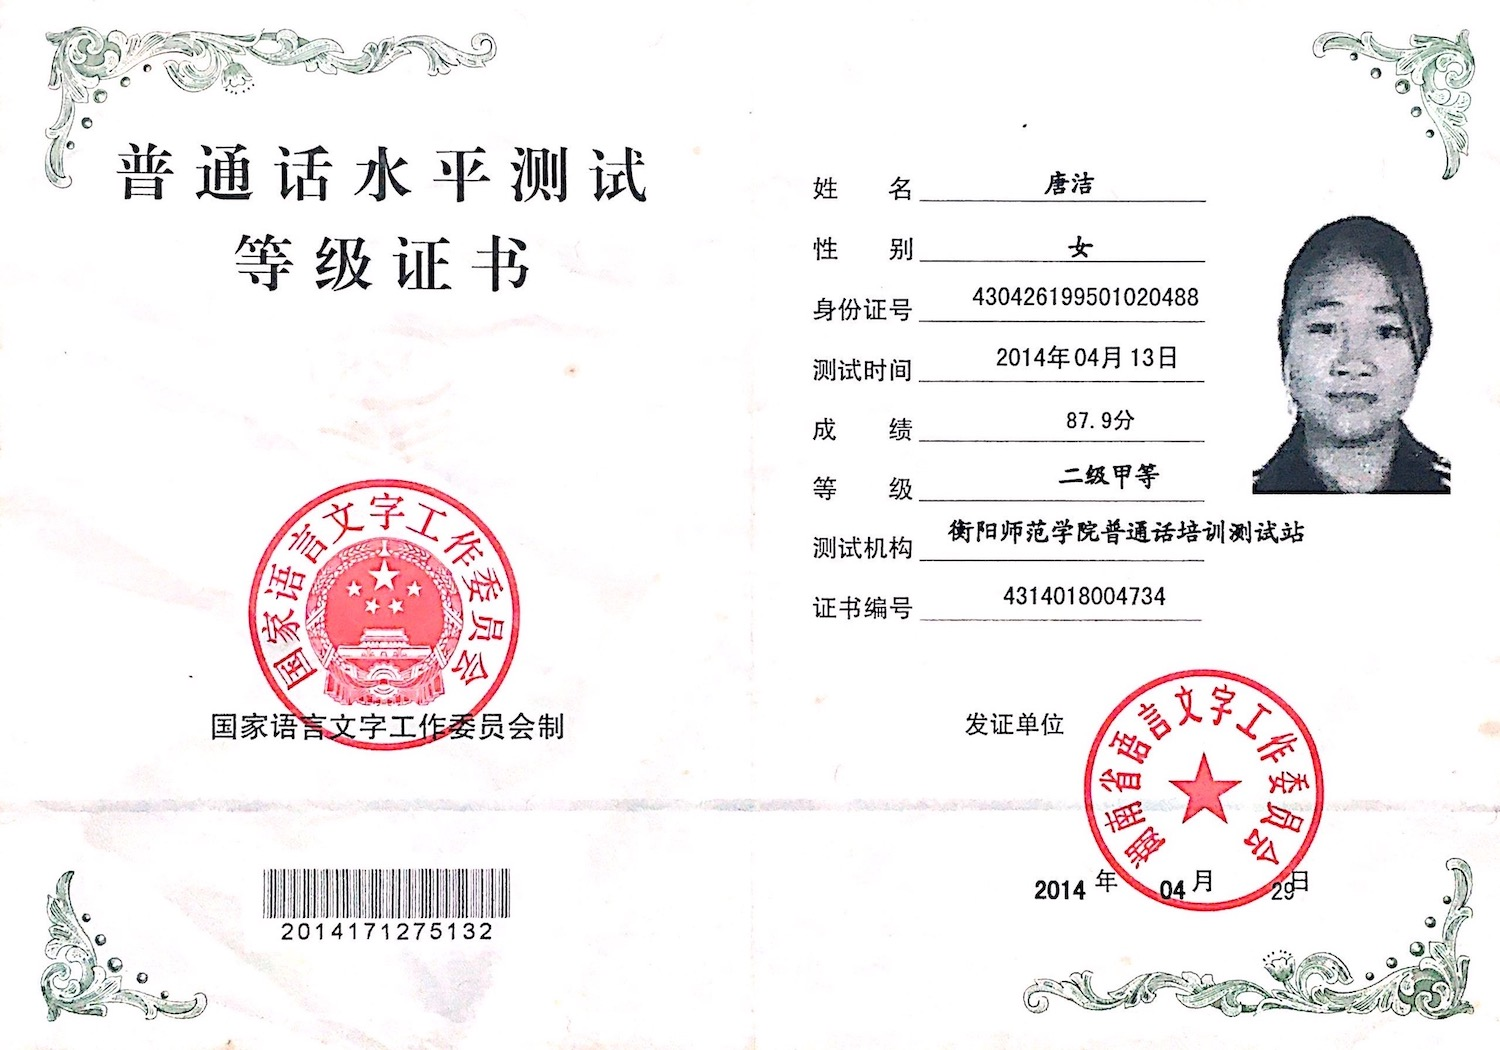
\includegraphics[scale=0.26]{figs/普通话证.JPG }

英语六级

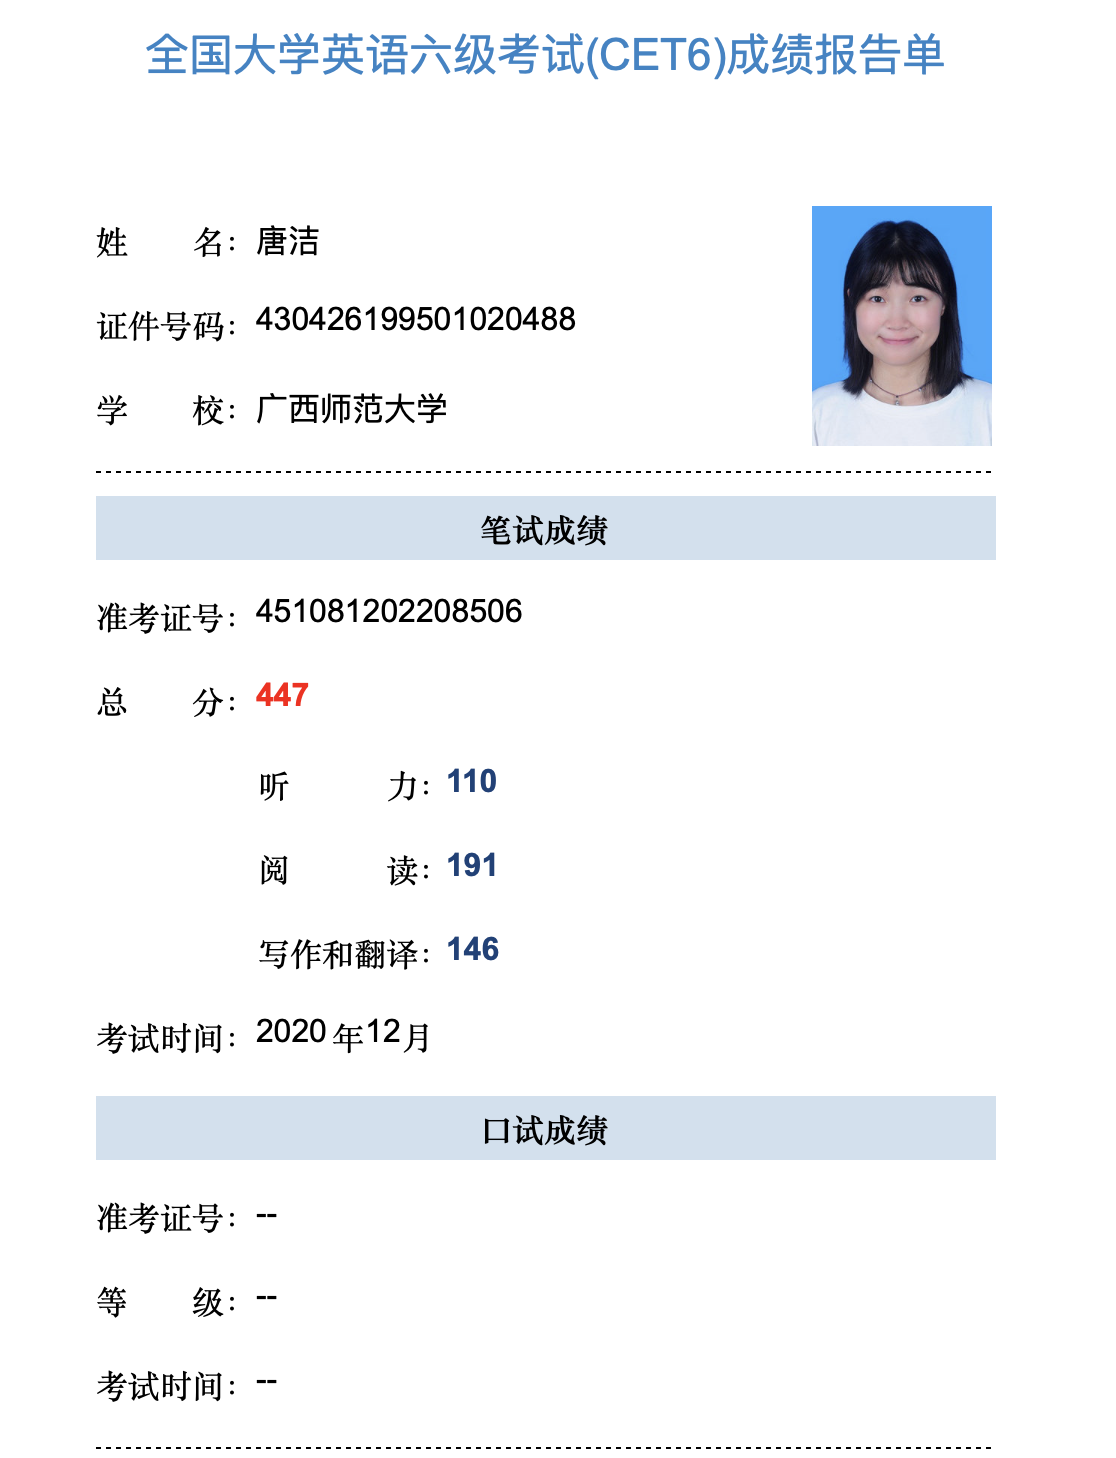
\includegraphics[scale=0.3]{figs/英语六级.JPG }
\end{center}

\section{荣誉证书}
\begin{center}
 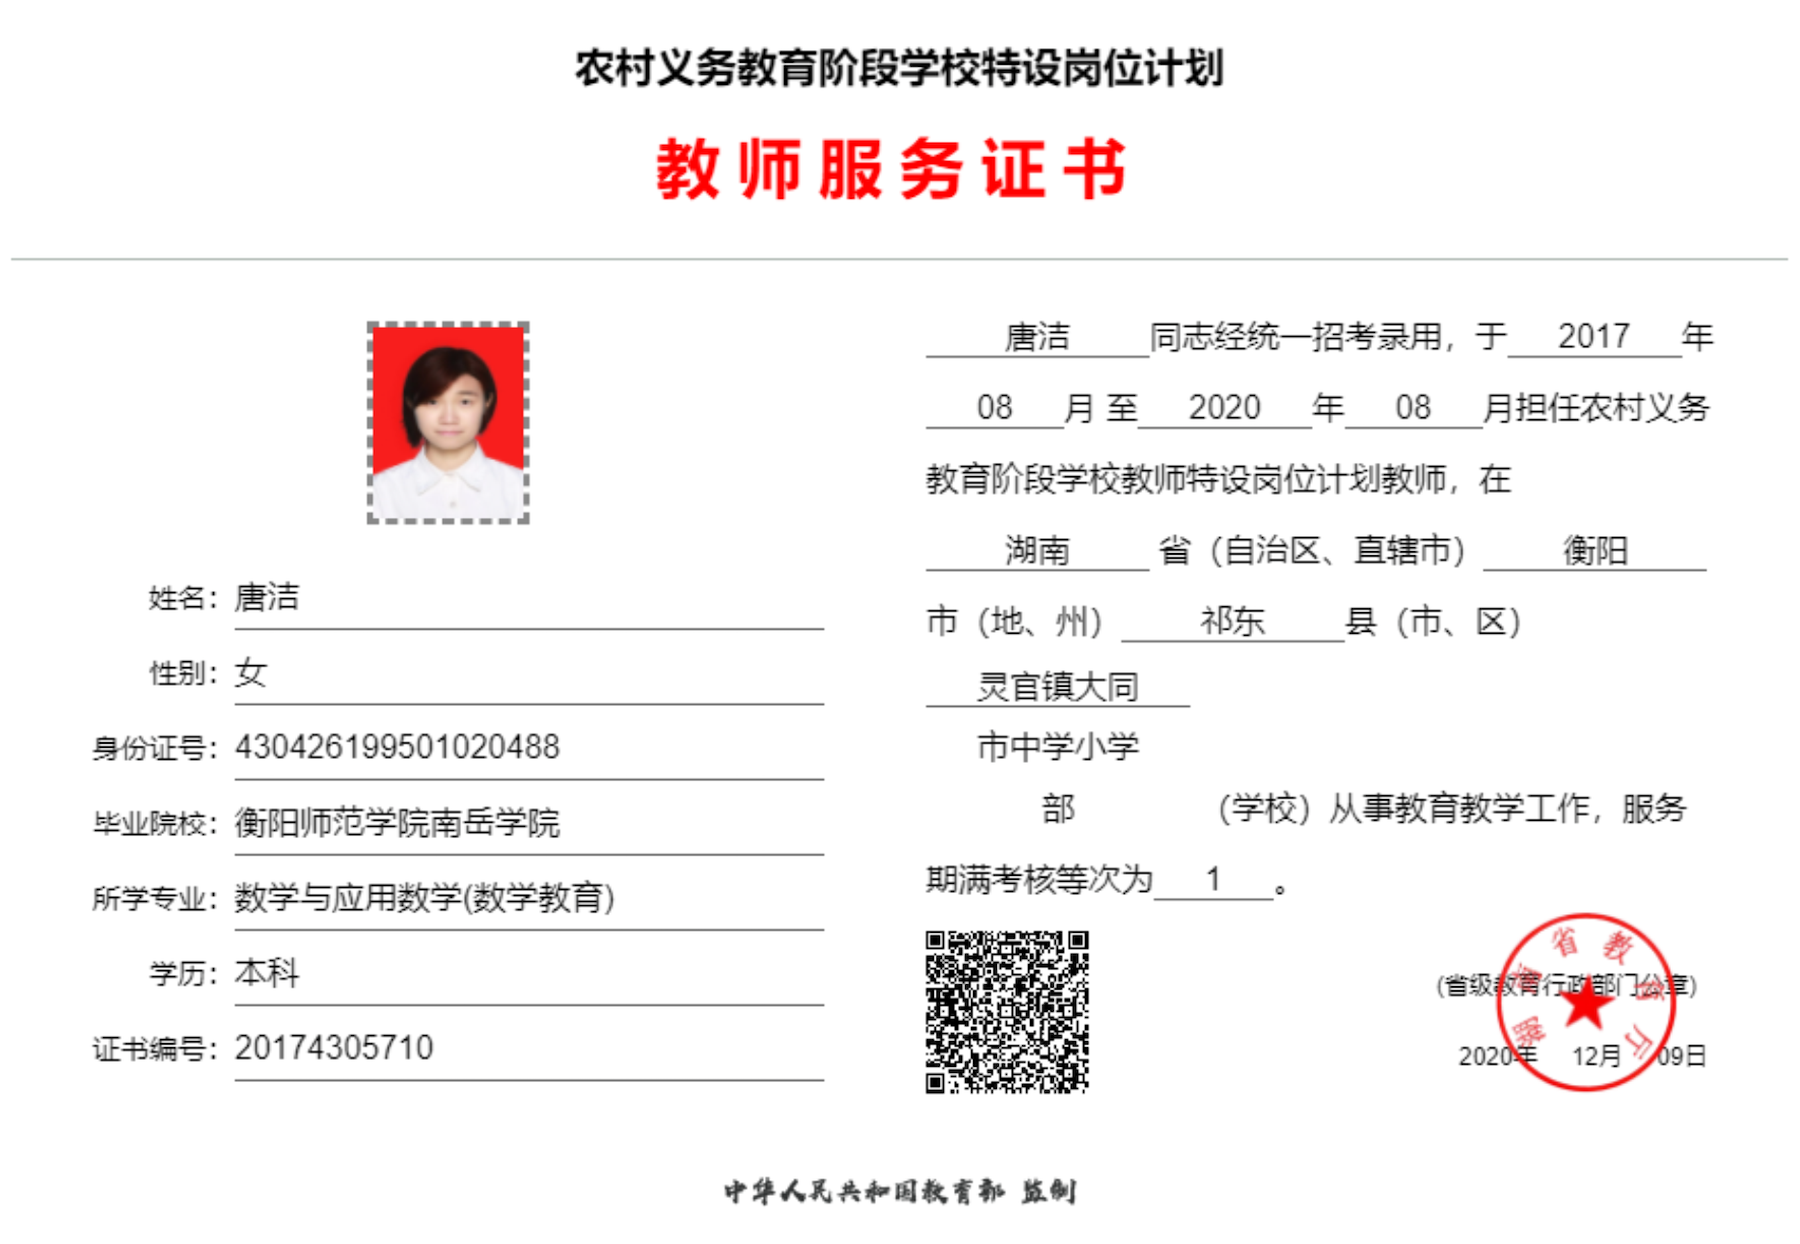
\includegraphics[scale=0.2]{figs/特岗服务证书.JPG }
 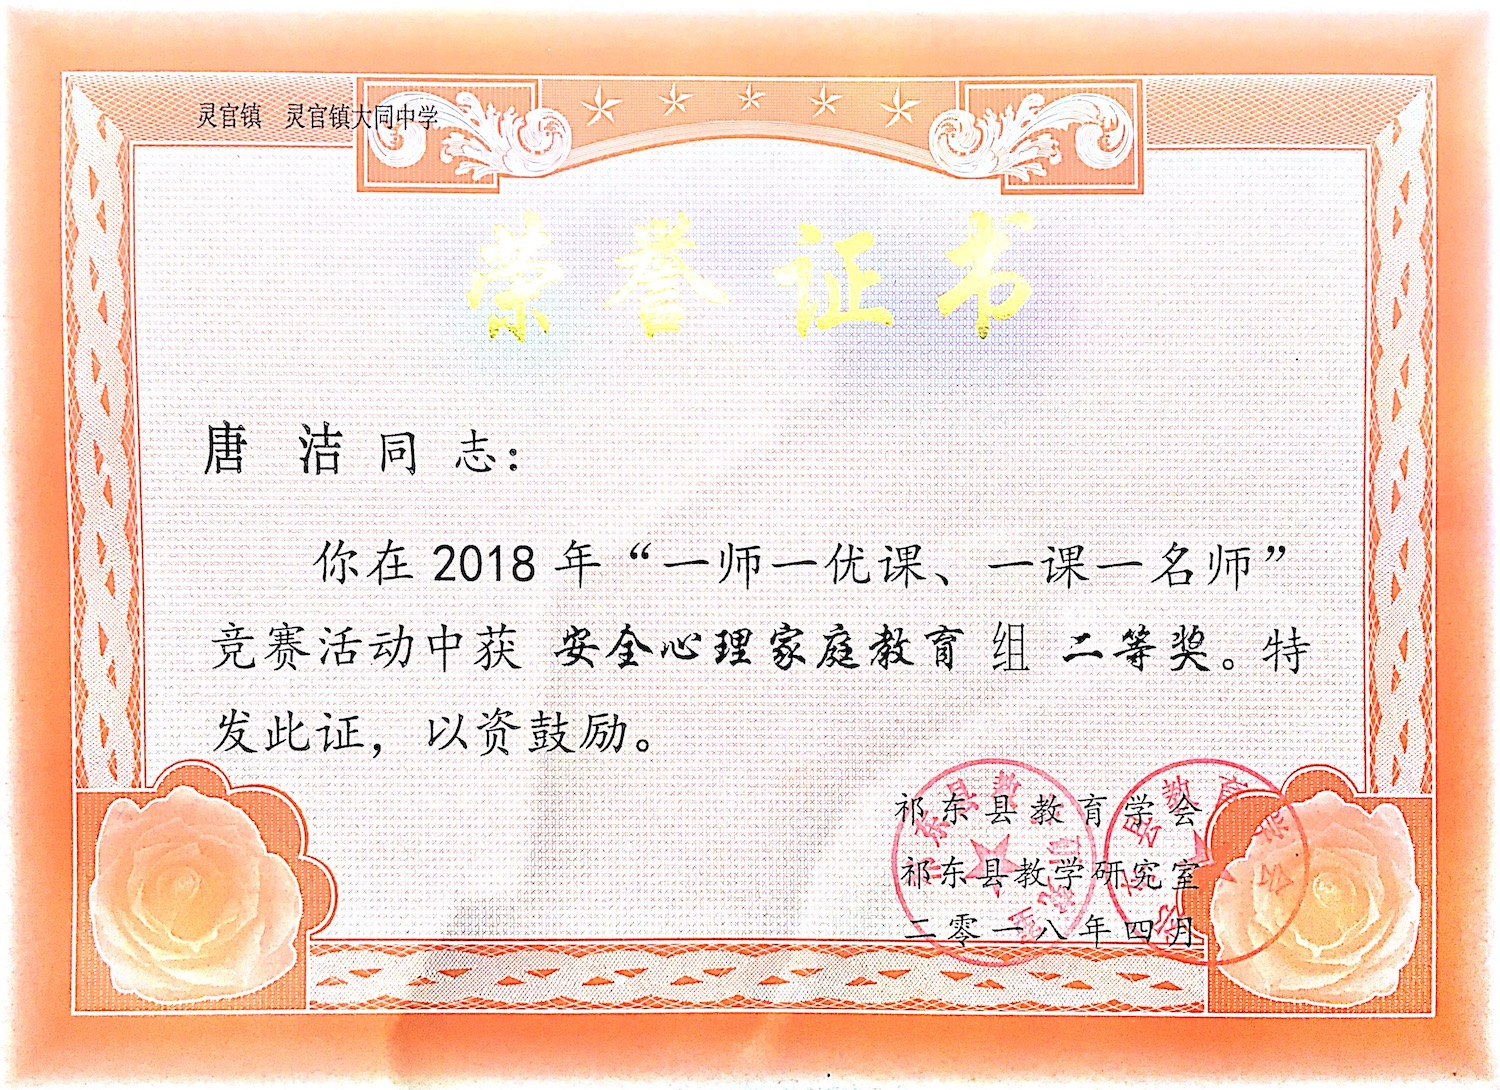
\includegraphics[scale=0.25]{figs/201804.JPG }
 
\includegraphics[scale=0.25]{figs/20180517.JPG }
 
\includegraphics[scale=0.16]{figs/201706.JPG }
% 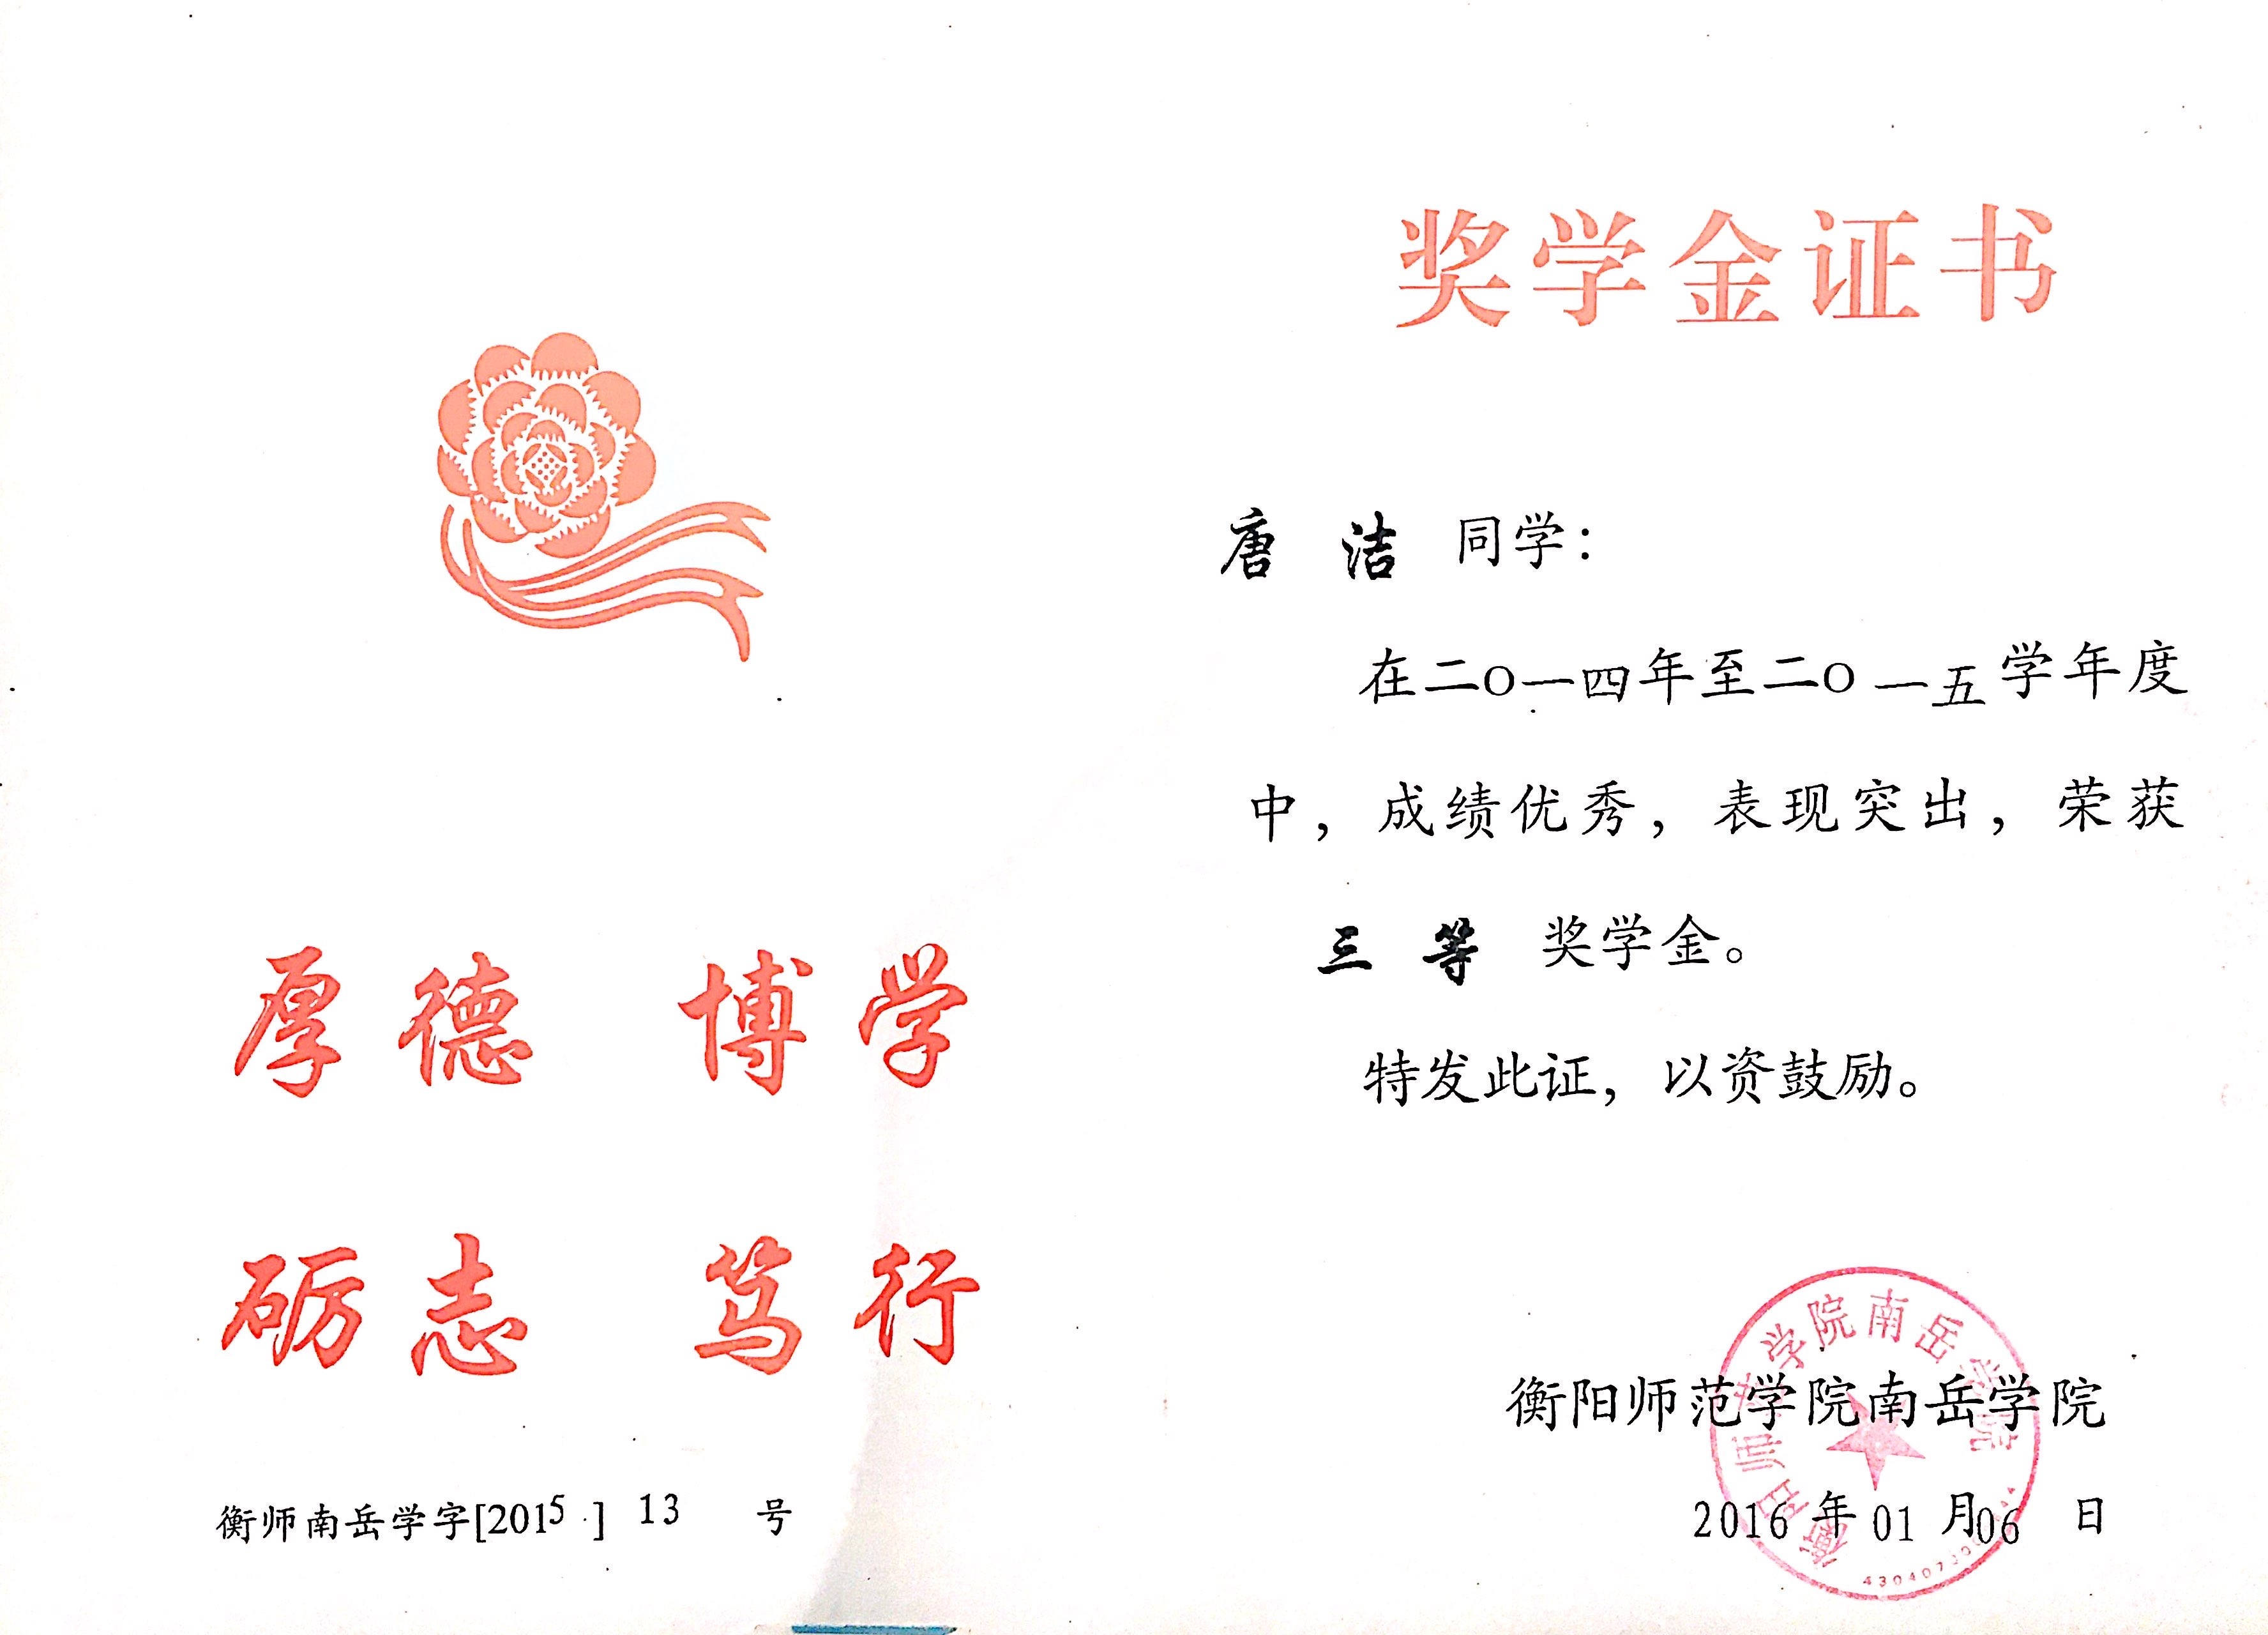
\includegraphics[scale=0.1]{figs/20160106.JPG }
% 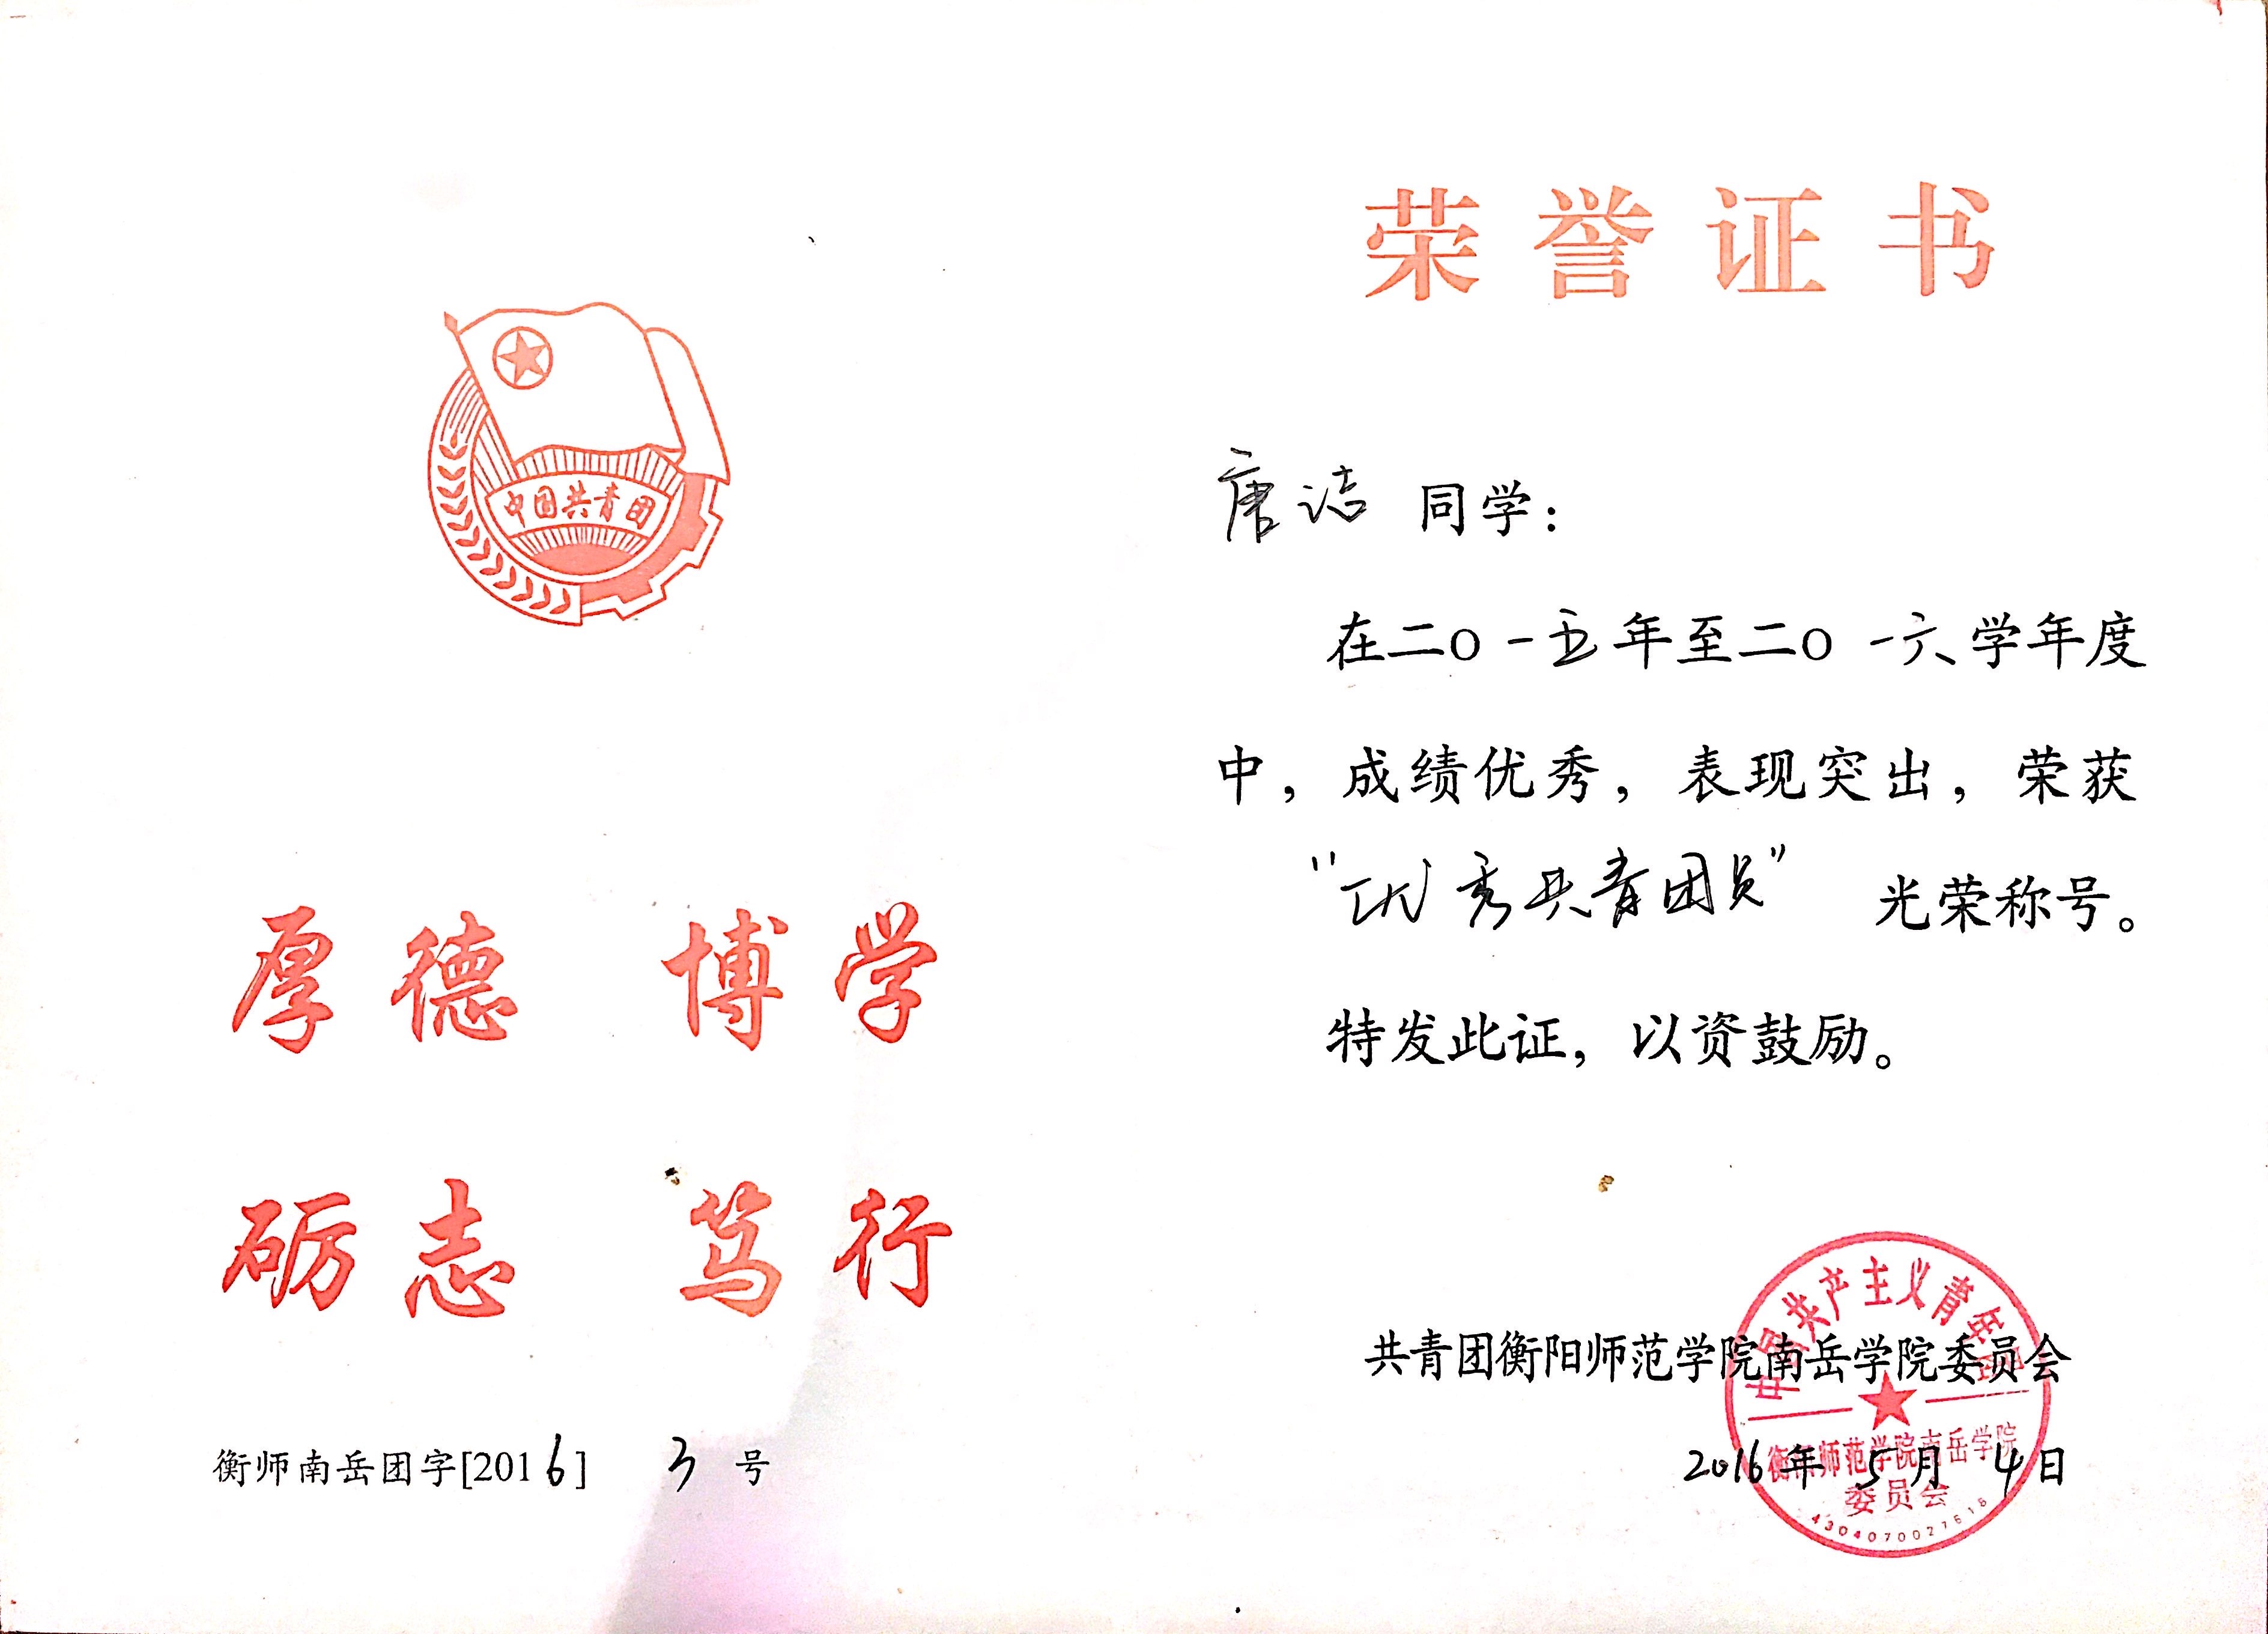
\includegraphics[scale=0.1]{figs/20160504.JPG }
% 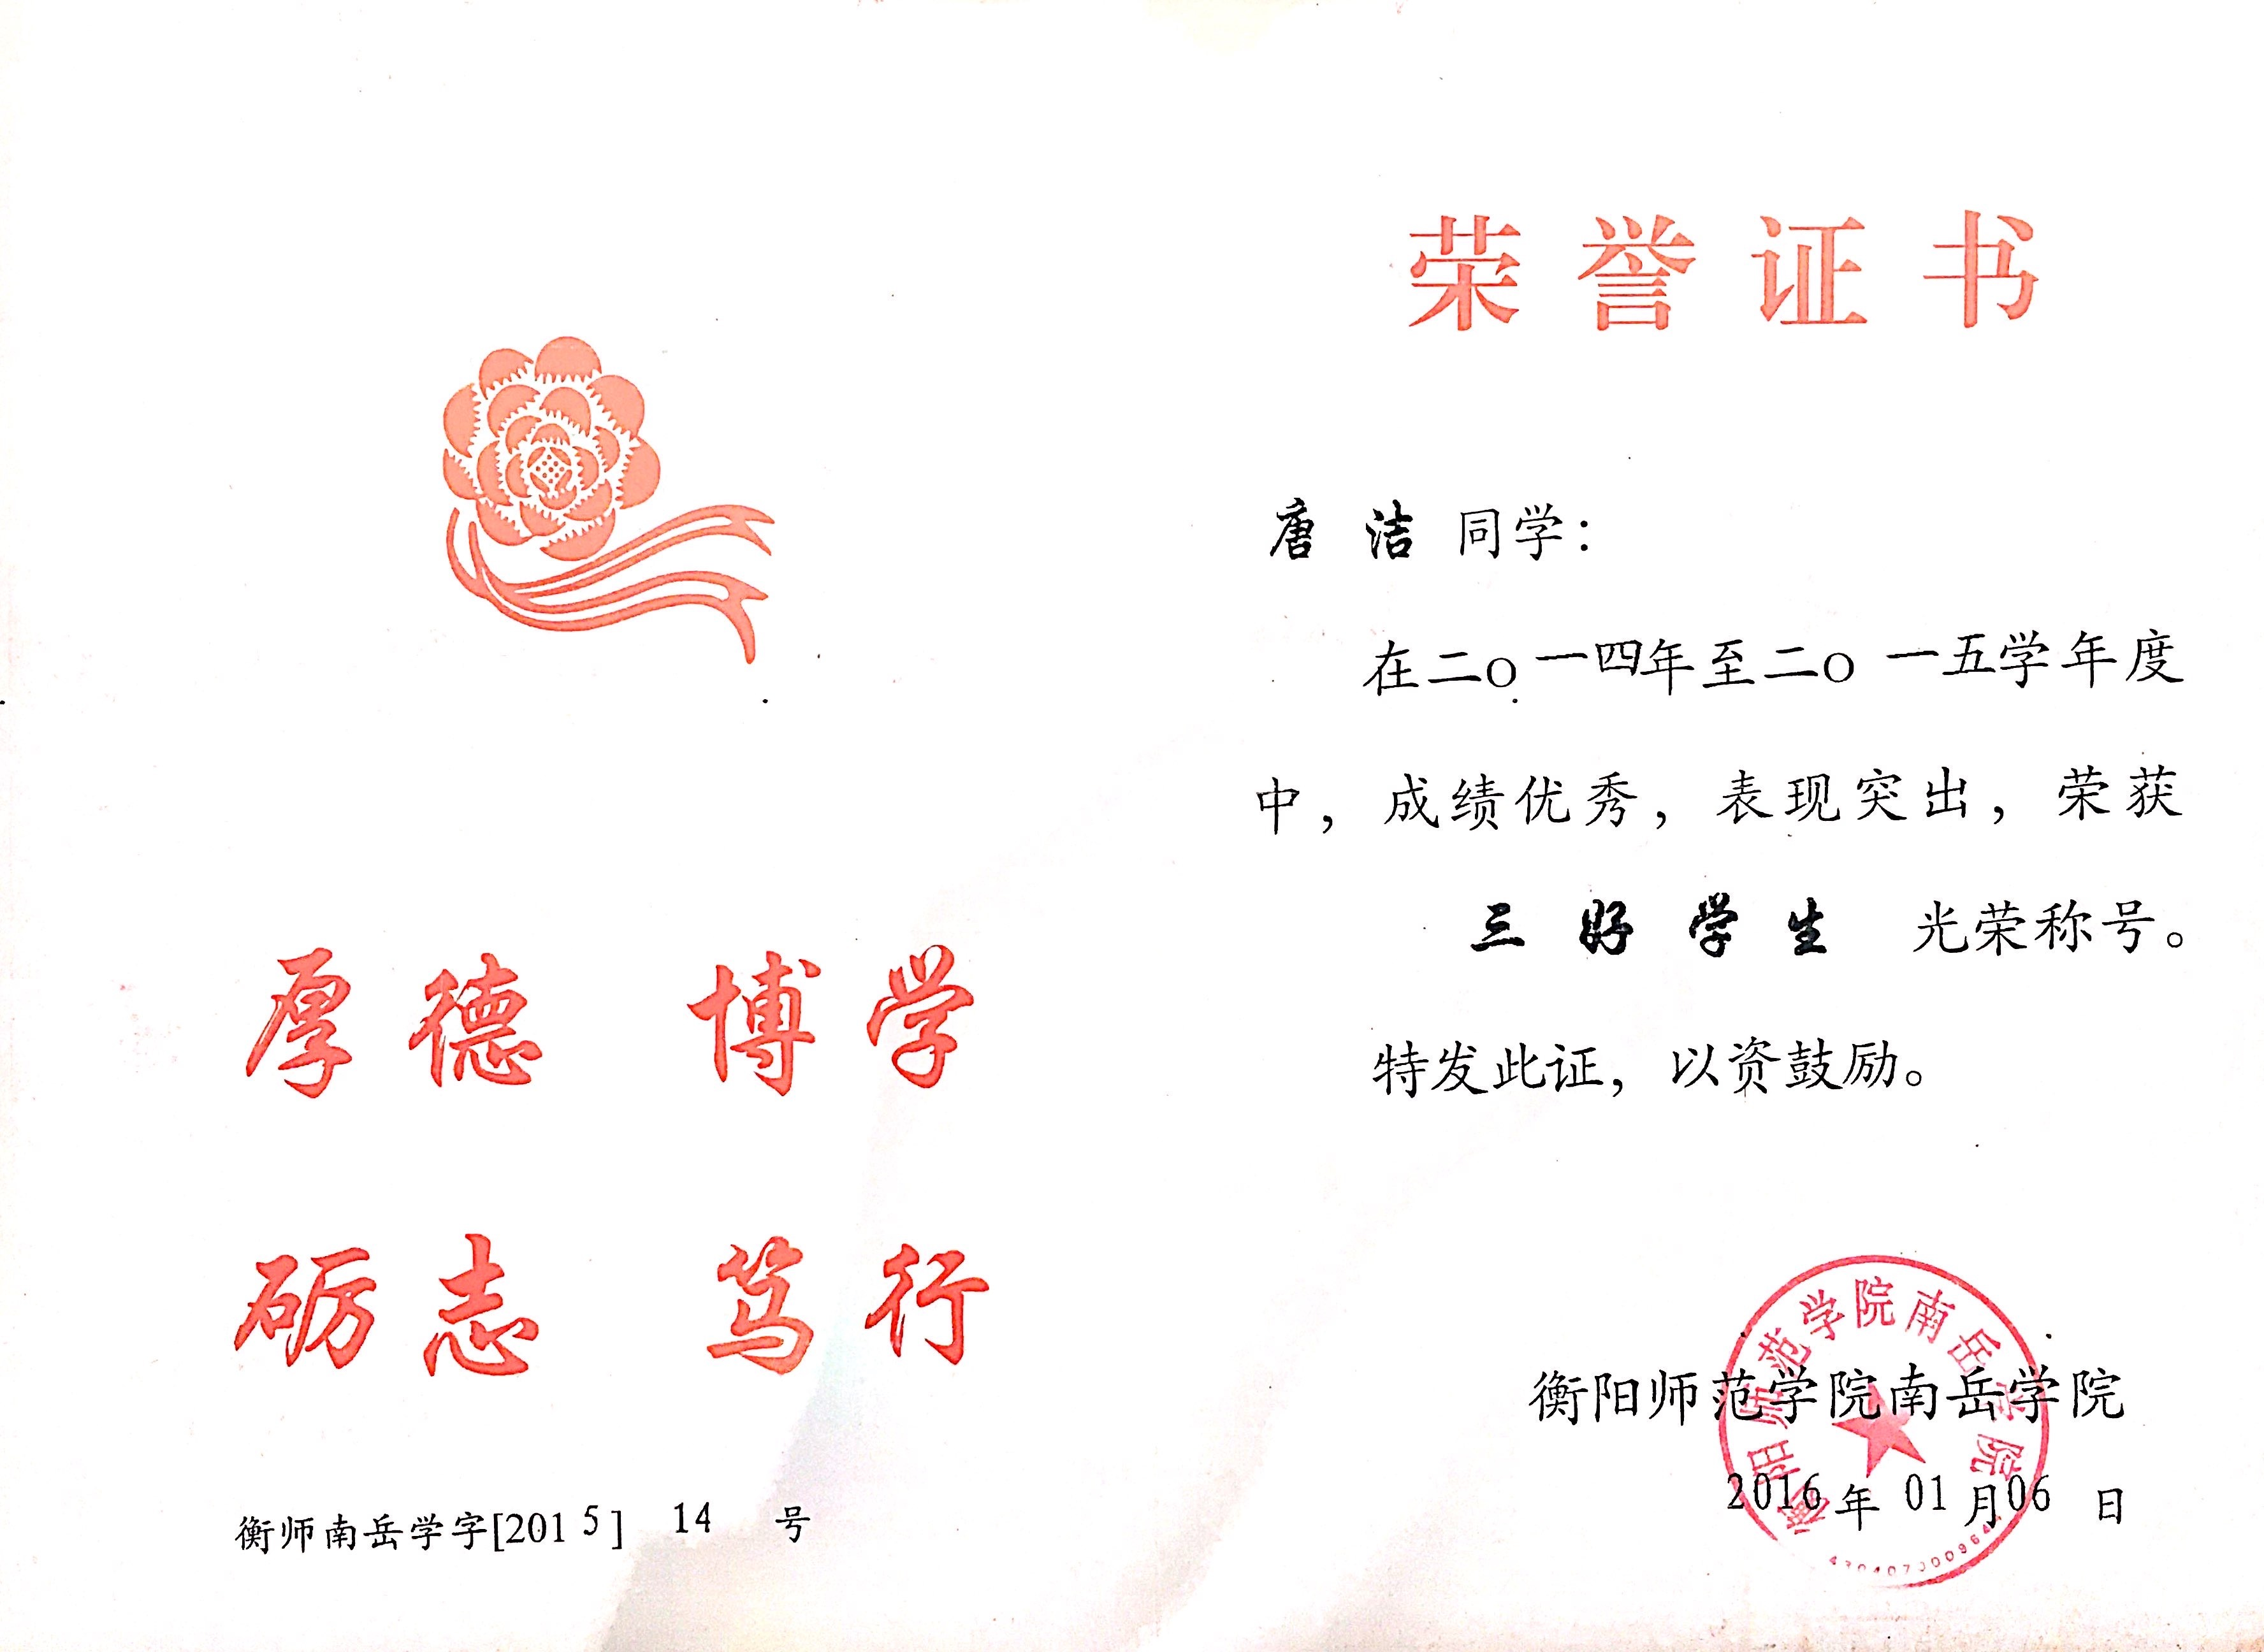
\includegraphics[scale=0.1]{figs/20160106_2.JPG }
\end{center}


\end{document}





